
\chapter{Classical Operads and Multicategories}
\lbl{ch:om}

\chapterquote{%
Some `pictures' are not really pictures, but rather are windows to Plato's%
%
\index{Plato}
%
heaven}{%
Brown~\cite{BrownJ}}

\noindent
Where category theory has arrows, higher-dimensional category theory has
higher-dimensional arrows.  One of the simplest examples of a
`higher-dimensional arrow' is one like
\[
\begin{centredpic}
\begin{picture}(6,4)(-1,-2)
\cell{0}{0}{l}{\tusual{}}
\cell{0}{0}{r}{\tinputsslft{}{}{}}
\cell{4}{0}{l}{\toutputrgt{}}
\end{picture}
\end{centredpic}
.
\]
Think of this as a box with $n$ input wires coming in on the left, where
$n$ is any natural number, and one output wire emerging on the right.  (For
instance, when $n=1$ this is just an arrow as in an ordinary category.)
With this in mind, it is easy to imagine what composition of such arrows
might look like: outputs of one arrow attach to inputs of another.

A categorical structure with arrows like this is called a multicategory.
(Multicategories and $n$-categories are not the same!)  A very familiar
example: the objects (drawn as labels on wires) are vector spaces, and the
arrows are multilinear maps.  The special case of a multicategory where
there is only one object---that is, the wires are unlabelled---is
particularly interesting.  Such a structure is called an operad; for a
basic example, fix a topological space $X$ and define an arrow with $n$
inputs to be a continuous map $X^n \go X$.

There is a curiously widespread impression that operads are frighteningly
complicated structures.  Among users of operads, there is a curiously
widespread impression that multicategories---usually known to them as
`coloured operads'---are some obscure and esoteric elaboration of the basic
notion of operad.  I hope this chapter will correct both impressions.  Both
structures are as natural as can be, and, if one draws some pictures, very
simple to understand.

We start with multicategories~(\ref{sec:cl-mtis}) then specialize to
operads~(\ref{sec:cl-opds}).  (This order of presentation may convince
sceptical operad-theorists that multicategories are natural structures in
their own right.)  The basic definitions are given, with a broad range of
examples.  An assortment of further topics on operads and multicategories
is covered in~\ref{sec:om-further}.

\paragraph*{Warning}%
%
\lbl{p:sym-warning}\index{operad!usage of word}\index{operad!symmetric}  
% 
Readers already familiar with operads may be used to them coming equipped
with symmetric group actions.  In this text operads \emph{without}
symmetries are the default.  This is partly to fit with the convention that
monoidal categories are by default non-symmetric, and rings, groups and
monoids non-commutative, but is mostly for reasons that will emerge later.
So:
%
\begin{quote}\centering\bf
`Operad' means what is sometimes called `non-$\Sigma$ operad' or
`non-symmetric operad'.
\end{quote}
% 
Operads equipped with symmetries will be called `symmetric operads'.


\section{Classical multicategories}
\lbl{sec:cl-mtis}%


Let us make the description above more precise.  
% 
A category consists of objects, arrows between objects, and a way of
composing arrows.  Precisely the same description applies to
multicategories.  The only difference 
% between the two structures
lies in the shape of the arrows: in a category, an arrow looks like
\[
a \goby{\theta} b,
\]
with one object as its domain and one object as its codomain, whereas in a
multicategory, an arrow looks like
%
\begin{equation}	\label{diag:multi-trans-arrow}
\begin{centredpic}
\begin{picture}(8,4)(-2,-2)
\cell{0}{0}{l}{\tusual{\theta}}
\cell{0}{0}{r}{\tinputsslft{a_1}{a_2}{a_n}}
\cell{4}{0}{l}{\toutputrgt{a}}
\end{picture}
\end{centredpic}
\end{equation}
%
($n\in\nat$), with a finite sequence of `input' objects as its domain and one
`output' object as its codomain.  
% Put another way, an arrow in a multicategory has
% several inputs and a single output.  
Arrows can be composed when outputs
are joined to inputs, which for categories means that any string of arrows
\[
a_0 \goby{\theta_1} a_1 \goby{\theta_2} 
\diagspace \cdots \diagspace
\goby{\theta_n} a_n
\]
has a well-defined composite, and for multicategories means (more
interestingly in geometrical terms) that any tree of arrows such as that in
Fig.~\ref{fig:random-multi-diagram}
%
\begin{figure}	
% \[
\begin{center}
\setlength{\unitlength}{1em}
\begin{picture}(24,13)(0,-5)
% transistors
\cell{18}{0}{l}{\tusual{\theta_1}}
\cell{10}{6}{l}{\tusual{\theta_2}}
\cell{10}{0}{l}{\tusual{\theta_3}}
\cell{2}{3}{l}{\tusual{\theta_4}}
\cell{2}{-3}{l}{\tusual{\theta_5}}
% short wires
\cell{22}{0}{l}{\toutputrgt{a_1}}
\cell{10}{7}{r}{\tinputlft{a_3}}
\cell{10}{5}{r}{\tinputlft{a_4}}
\cell{2}{-1.5}{r}{\tinputlft{a_8}}
\cell{2}{-3}{r}{\tinputlft{a_9}}
\cell{2}{-4.5}{r}{\tinputlft{a_{10}}}
\cell{18}{-1.5}{r}{\tinputlft{a_{11}}}
% long wires
\qbezier(18,1.5)(16.5,1.5)(16,3.75)
\qbezier(14,6)(15.5,6)(16,3.75)
\cell{16.5}{3.75}{l}{a_2}
\put(18,0){\line(-1,0){4}}
\cell{16}{0.2}{b}{a_5}
\qbezier(10,1)(8.5,1)(8,2)
\qbezier(6,3)(7.5,3)(8,2)
\cell{8.5}{2}{l}{a_6}
\qbezier(10,-1)(8.5,-1)(8,-2)
\qbezier(6,-3)(7.5,-3)(8,-2)
\cell{8.5}{-2}{l}{a_7}
\end{picture}
\end{center}
% \hand{45}{50}
% \]
\caption{Composable diagram of arrows in a multicategory}
\label{fig:random-multi-diagram}
\end{figure}
%
has a well-defined composite, in this case of the form
\[
\begin{centredpic}
\begin{picture}(10,6)(-2,-3)
% transistor
\cell{0}{0}{l}{\tmid{}}
% tags
\cell{0}{2.5}{r}{\tinputlft{a_3}}
\cell{0}{1.5}{r}{\tinputlft{a_4}}
\cell{0}{0.5}{r}{\tinputlft{a_8}}
\cell{0}{-0.5}{r}{\tinputlft{a_9}}
\cell{0}{-1.5}{r}{\tinputlft{a_{10}}}
\cell{0}{-2.5}{r}{\tinputlft{a_{11}}}
\cell{6}{0}{l}{\toutputrgt{a_1.}}
\end{picture}
\end{centredpic}
\]
Perhaps the most familiar example is where the objects are vector spaces
and the arrows are multilinear maps.  Commonly the multicategory structure
is obscured by the device of considering multilinear maps as linear maps
out of a tensor product; but in many situations it is the multicategory,
not the monoidal category, that is fundamental.

\begin{defn}	\lbl{defn:cl-multi}
A \demph{multicategory}%
%
\index{multicategory}
%
$C$ consists of
%
\begin{itemize}
\item a class $C_0$,%
% 
\glo{C0multicat}
% 
whose elements are called the \demph{objects} of $C$
\item for each $n\in\nat$ and $a_1, \ldots, a_n, a \in C_0$, a class
$C(a_1, \ldots, a_n; a)$,%
% 
\glo{multicathomset}
% 
whose elements $\theta$ are called \demph{arrows}
or \demph{maps} and depicted as in~\bref{diag:multi-trans-arrow} or as
%
\begin{equation}	\label{eq:multi-arrow}
a_1, \ldots, a_n \goby{\theta} a
\end{equation}
%
\item for each $n, k_1, \ldots, k_n \in \nat$ and $a, a_i, a_i^j \in C_0$,
a function (Fig.~\ref{fig:multi-comp})
\[
\begin{array}{r}
C(a_1, \ldots, a_n; a) \times
C(a_1^1, \ldots, a_1^{k_1}; a_1) \times \cdots \times
C(a_n^1, \ldots, a_n^{k_n}; a_n)\\
\go
C(a_1^1, \ldots, a_1^{k_1}, \ldots, a_n^1, \ldots, a_n^{k_n}; a),
\end{array}
\]
called \demph{composition} and written
\[
(\theta, \theta_1, \ldots, \theta_n) \goesto 
\theta \of (\theta_1, \ldots, \theta_n)
% 
\glo{multicomposite}%
\]%
% 
\item for each $a\in C_0$, an element $1_a \in C(a;a)$,%
% 
\glo{multiidentity}
% 
called the
\demph{identity} on $a$
\end{itemize}
%
satisfying
%
\begin{itemize}
\item associativity:
%
\begin{eqnarray*}
&&\theta \of 
\left(
\theta_1 \of (\theta_1^1, \ldots, \theta_1^{k_1}),
\ldots,
\theta_n \of (\theta_n^1, \ldots, \theta_n^{k_n})
\right)\\
&=&
\left(\theta \of (\theta_1, \ldots, \theta_n)\right) \of
(\theta_1^1, \ldots, \theta_1^{k_1}, 
\ldots, 
\theta_n^1, \ldots, \theta_n^{k_n})
\end{eqnarray*}
%
whenever $\theta, \theta_i, \theta_i^j$ are arrows for which these
composites make sense
\item identity:
\[
\theta \of (1_{a_1}, \ldots, 1_{a_n}) 
= 
\theta 
= 
1_a \of (\theta)
\]
whenever $\theta: a_1, \ldots, a_n \go a$ is an arrow.
\end{itemize}
\end{defn}
%
\begin{figure}
\[
% DOMAIN
%
\begin{centredpic}
\begin{picture}(16.5,12)(-0.5,-6)
% transistors
\cell{10}{0}{l}{\tusual{\theta}}
\cell{2}{4}{l}{\tusual{\theta_1}}
\cell{2}{-4}{l}{\tusual{\theta_n}}
% short wires
\cell{14}{0}{l}{\toutputrgt{a}}
\cell{2}{4}{r}{\tinputslft{a_1^1}{a_1^{k_1}}}
\cell{2}{-4}{r}{\tinputslft{a_n^1}{a_n^{k_n}}}
% long wires
\qbezier(10,1.5)(8.5,1.5)(8,2.75)
\qbezier(6,4)(7.5,4)(8,2.75)
\cell{8.5}{2.75}{l}{a_1}
\qbezier(10,-1.5)(8.5,-1.5)(8,-2.75)
\qbezier(6,-4)(7.5,-4)(8,-2.75)
\cell{8.5}{-2.75}{l}{a_n}
% ellipses
\cell{9.2}{0.3}{c}{\vdots}
\cell{3}{0}{c}{\cdot}
\cell{3}{1}{c}{\cdot}
\cell{3}{-1}{c}{\cdot}
\end{picture}
\end{centredpic}
%
\mbox{\hspace{2em}}
\goesto
\mbox{\hspace{2em}}
%
% CODOMAIN
%
\begin{centredpic}
\begin{picture}(10,12)(0,-6)
% transistor
\put(2,-6){\line(0,1){12}}
\put(8,0){\line(-1,-1){6}}
\put(8,0){\line(-1,1){6}}
\cell{5}{0}{c}{\scriptstyle\theta \sof (\theta_1, \ldots, \theta_n)}
% \cell{5}{0}{c}{\theta \circ (\theta_1, \ldots, \theta_n)}
% tags
\cell{2}{4}{r}{\tinputslft{a_1^1}{a_1^{k_1}}}
\cell{2}{-4}{r}{\tinputslft{a_n^1}{a_n^{k_n}}}
\cell{1.2}{0.3}{c}{\vdots}
\cell{8}{0}{l}{\toutputrgt{a}}
\end{picture}
\end{centredpic}
\]
% \hand{50}{51}
\caption{Composition in a multicategory}
\label{fig:multi-comp}
\end{figure}

Operads are precisely multicategories with only one object, and are the
subject of the next section.  For now we look at multicategories with many
objects---often a proper class of them.

\begin{example}	\lbl{eg:multi-unary}
A multicategory in which every arrow is \demph{unary}%
%
\index{unary}
%
(that is, of the
form~\bref{eq:multi-arrow} with $n=1$) is the same thing as a category. 
\end{example}

\begin{example}	\lbl{eg:multi-mon}%
Any monoidal category $(A, \otimes)$ has an \demph{underlying
multicategory}%
%
\index{multicategory!underlying}
%
 $C$.  It has the same objects as $A$, and a map
\[
a_1, \ldots, a_n \go a
\]
in $C$ is a map
\[
a_1 \otimes \cdots \otimes a_n \go a
\]
in $A$.  Composition in $C$ is derived from composition and tensor in $A$.

If $A$ is a non-strict monoidal category then there is some ambiguity in
the meaning of `$a_1 \otimes\cdots\otimes a_n$'.  We will address this
properly in~\ref{sec:non-alg-notions}, but for now let us just choose
a particular bracketing, e.g.\ $((a_1 \otimes a_2) \otimes a_3) \otimes
a_4$ for $n=4$.

Given a commutative ring $R$, the monoidal category of $R$-modules%
%
\index{module!ring@over ring}
%
with their usual tensor gives rise in this way to a multicategory of
$R$-modules and $R$-multilinear maps.  Similarly, given a category $A$ with
finite products there is an underlying multicategory $C$ with the same
objects as $A$ and with
\[
C(a_1, \ldots, a_n; a) = A(a_1 \times\cdots\times a_n, a).
\]
We will make particular use of the multicategory $C$ coming from the
category $A = \Set$;%
%
\index{multicategory!sets@of sets}
%
we write $C = \Set$ too.
\end{example}

\begin{example}	\lbl{eg:multi-some-of-mon}
More generally, if $A$ is a monoidal category and $C_0$ a collection of
objects of $A$ (not necessarily closed under tensor) then there is a
multicategory $C$ whose class of objects is $C_0$ and whose arrows are
defined as in the previous example. 
\end{example}

It is important to realize that \emph{not} every multicategory%
%
\lbl{p:not-ESO}
%
is the underlying%
%
\index{multicategory!underlying}
%
multicategory of a monoidal
category~(\ref{eg:multi-mon}).  Example~\ref{eg:multi-some-of-mon} makes
this reasonably clear.  Another way of seeing it is to consider one-object
multicategories (operads, next section): if $A$ is a monoidal category with
single object $a$ then in the underlying multicategory $C$, the cardinality
of the hom-set $C(a, \ldots, a; a)$ is independent of the number of $a$'s
in the domain.  But this independence property certainly does not hold for
all one-object multicategories, as numerous examples in
Section~\ref{sec:cl-opds} show.


\begin{example}%
%
\index{multicategory!underlying}
%
Sometimes tensor is irrelevant; sometimes it does not even exist.  For
instance, let $V$ be a symmetric monoidal category and let $\Ab(V)$ be the
category of abelian groups in $V$.  In general $V$ will not have enough
colimits to define a tensor product on $\Ab(V)$ and so make it into a
monoidal category.  But it is always possible to define multilinear maps
between abelian groups in $V$, giving $\Ab(V)$ the structure of a
multicategory.
\end{example}

\begin{example}	\lbl{eg:multi-pretend-coproducts}
If $A$ is a category with finite coproducts%
%
\index{operad!coproducts@from coproducts}
%
then Example~\ref{eg:multi-mon}
reveals that there is a multicategory $C$ with the same objects as $A$,
with
\[
C(a_1, \ldots, a_n; a)
=
% A(a_1 + \cdots + a_n, a)
% \iso
A(a_1, a) \times\cdots\times A(a_n, a),
\]
and with composition given by
%
\begin{eqnarray*}
&&
(f_1, \ldots, f_n) \of 
((f_1^1, \ldots, f_1^{k_1}), \ldots, (f_n^1, \ldots,  f_n^{k_n}))\\
&=&
(f_1 \of f_1^1, \ldots, f_1 \of f_1^{k_1}, \ldots,
f_n \of f_n^1, \ldots, f_n \of f_n^{k_n})
\end{eqnarray*}
%
($f_i \in A(a_i, a)$, $f_i^j \in A(a_i^j, a_i)$).  Indeed, these formulas
make sense and define a multicategory $C$ for any category $A$ whatsoever.
An arrow of $C$ can be drawn as
\[
\begin{centredpic}
\begin{picture}(10,6)(0,-3)
% transistor
\cell{2}{0}{l}{\tmid{}}
% tags
\cell{2}{2}{r}{\tinputlft{a_1}}
\cell{2}{1}{r}{\tinputlft{a_2}}
\cell{2}{-2}{r}{\tinputlft{a_n}}
\cell{8}{0}{l}{\toutputrgt{a.}}
% lines inside transistor...
\qbezier(2,2)(5,1)(8,0)
\qbezier(2,1)(5,0.5)(8,0)
\qbezier(2,-2)(5,-1)(8,0)
% ...and their arrowheads
\cell{3.5}{1.4}{br}{\rotatebox{35}{$\lrcorner$}}
\cell{3.5}{0.6}{br}{\rotatebox{30}{$\lrcorner$}}
\cell{3.5}{-1.3}{tr}{\rotatebox{70}{$\lrcorner$}}
% ...and their labels
\cell{3}{2.1}{c}{\scriptstyle f_1}
\cell{3}{0.4}{c}{\scriptstyle f_2}
% \cell{3}{-1.3}{c}{\scriptstyle f_n}
\cell{3}{-2}{c}{\scriptstyle f_n}
% ellipses
\cell{1.2}{-.3}{c}{\vdots}
\cell{4}{-0.1}{c}{\vdots}
\end{picture}
\end{centredpic}
% \hand{30}{52}.
\]
\end{example}


\begin{example}
A category in which each hom-set has at most one element is the same thing
as a preordered%
%
\index{order!generalized}%
%
\index{multicategory!poset-like}
%
set.  Similarly, a multicategory $C$ in which $C(a_1,
\ldots, a_n; a)$ has at most one element for each $n, a_1, \ldots, a_n, a$
is some kind of generalized poset.  It amounts to a class $X = C_0$ of
elements together with an $(n+1)$-ary relation $\leq_n$ on $X$
%  \sub X^n \times X$
for each $n\in\nat$, satisfying generalized reflexivity and transitivity
axioms.  For instance, let $d\in\nat$, let $X = \reals^d$, and define
$\leq_n$ by $(a_1, \ldots, a_n) \leq_n a$ if and only if $a$ is in the
convex%
%
\index{convex hull}
%
hull of $\{ a_1, \ldots, a_n \}$.  This gives a `generalized poset';
the axioms express basic facts about convex hulls.
\end{example}

The final example is more substantial.

\begin{example}	\lbl{eg:multi-cheese}
The \demph{Swiss%
%
\index{multicategory!Swiss cheese}
%
cheese multicategory} $\fcat{SC}$ has the natural numbers
as its objects, with $d\in\nat$ thought of as the $d$-dimensional disk.
Maps are configurations of disks, half-disks, quarter-disks, and so on, as
now described.

Let $\reals^\infty$ be the set of sequences $(x_n)_{n=1}^{\infty}$ of real
numbers.  For each $d\in\nat$, let
\[
\cheesydisk{d} = 
\{ \mathbf{x} \in \reals^\infty
\such
\sum_{n=1}^{\infty} x_n^2 \leq 1 
\textrm{, and } x_n \geq 0 \textrm{ for all } n>d \},
\]
and define a sequence of subsets $F^d_1, F^d_2, \ldots$ of $\cheesydisk{d}$
by
\[
F^d_n =
\left\{
\begin{array}{ll}
\emptyset	&\textrm{ if } n\leq d	\\
\{ \mathbf{x} \in \cheesydisk{d}
\such
x_n = 0 \}	&\textrm{ if } n>d.
\end{array}
\right.
\]
(The idea is that if the hyperplane $x_n = 0$ contains one of the flat
faces of $\cheesydisk{d}$ then $F^d_n$ is that flat face, and otherwise
$F^d_n$ is empty.)  Let $G$ be the group of bijections on $\reals^\infty$
of the form $\mathbf{x} \goesto \mathbf{a} + \lambda\mathbf{x}$ for some
$\mathbf{a} \in \reals^\infty$ and $\lambda > 0$.  Then there is a category
$A$ in which the objects are the natural numbers and a map $d' \go d$ is an
element $\alpha\in G$ such that
\[
\alpha\cheesydisk{d'} \sub \cheesydisk{d},
\diagspace
\alpha F^{d'}_n \sub F^d_n \textrm{ for all } n\geq 1.
\]
(So $\alpha$ sends $\cheesydisk{d'}$ into $\cheesydisk{d}$, with flat faces
mapping into flat faces.)  By Example~\ref{eg:multi-pretend-coproducts},
there arises a multicategory $C$ with object-set $\nat$ and with
\[
C(d_1, \ldots, d_k; d) = A(d_1, d) \times\cdots\times A(d_k, d).
\]
The Swiss cheese multicategory $\fcat{SC}$ is the sub-multicategory of $C$
consisting of the same objects but only those arrows
\[
(\alpha_1, \ldots, \alpha_k) \in C(d_1, \ldots, d_k; d)
\]
for which the images $\alpha_i \cheesydisk{d_i}$ and $\alpha_j
\cheesydisk{d_j}$ are disjoint whenever $i\neq j$.  

A few calculations reveal that $\fcat{SC}(d_1, \ldots, d_k; d)$ is only
non-empty when $d_i \geq d$ for each $i$, and that the description of this
hom-set is unchanged if we replace $\reals^\infty$ by $\reals^{\max\{d_1,
\ldots, d_k\} }$ throughout.  It follows that, for instance, a map
\[
1, 1, 2, 2, 2, 3 \go 1
\]
(Fig.~\ref{fig:cheese}) 
%
\begin{figure}
\begin{center}
\setlength{\unitlength}{1mm}
\begin{picture}(104,70)
% cheese.eps is 72mm wide and 70mm high
\cell{0}{0}{bl}{\epsfig{file=cheese.eps}}
\cell{92}{35}{l}{\epsfig{file=cheeseaxes.eps}}
\cell{105}{23}{c}{x_1}
\cell{107}{36.5}{c}{x_2}
\cell{94}{47}{c}{x_3}
\end{picture}
\end{center}
% \hand{70}{53}
\caption{Swiss cheese map $1, 1, 2, 2, 2, 3 \protect\go 1$}
\label{fig:cheese}
\end{figure}
%
is a configuration of two quarter-balls, three half-balls, and one whole
ball inside the unit quarter-ball in $\reals^3$, with the (straight)
$1$-dimensional face of each quarter-ball lying on the $1$-dimensional face
of the unit quarter-ball and the (flat) $2$-dimensional face of each
half-ball lying on the 2-dimensional face $x_3=0$ of the unit quarter-ball.
The six little fractions of balls must be disjoint.

For each $d\in\nat$ there is a sub-multicategory $\fcat{SC}_d$ consisting
of only the two objects $d$ and $d+1$ (and all the maps between them).
This was Voronov's%
%
\index{Voronov, Alexander}
%
original `Swiss-cheese%
%
\index{operad!Swiss cheese}
%
operad' (a `2-coloured operad');
see Voronov~\cite{VorSCO} and Kontsevich~\cite[2.5]{KonOMD}.%
%
\index{Kontsevich, Maxim}
%
 The
one-object sub-multicategories of $\fcat{SC}$ are more famous: for each
$d\in\nat$, the sub-multicategory consisting of $d$ (and all maps) is
exactly the little%
%
\index{operad!little disks}
%
$d$-dimensional disks
operad~(\ref{eg:opd-little-disks}).
\end{example}


Many of the multicategories mentioned have a natural symmetric structure:
there is a bijection
\[
\dashbk\cdot\sigma:
C(a_1, \ldots, a_n; a)
\goiso
C(a_{\sigma(1)}, \ldots, a_{\sigma(n)}; a)
\]%
% 
\glo{dotsigma}%
% 
for each $a_1, \ldots, a_n, a \in C_0$ and permutation $\sigma\in S_n$.%
% 
\glo{symgp}
% 
 A
`symmetric%
%
\index{multicategory!symmetric}
%
multicategory'%
\lbl{p:sym-mti-informal}
%
is defined as a multicategory equipped with such a family of bijections,
satisfying axioms.  We give the precise definition in~\ref{defn:sym-mti};
see also Appendix~\ref{app:sym}.  For example, if $A$ is a symmetric
monoidal category then its underlying multicategory $C$ is also symmetric.

Similarly, many of these examples are also naturally `enriched':%
%
\lbl{p:sym-enr-mti}%
%
\index{enrichment!plain multicategory@of plain multicategory!symmetric monoidal category@in symmetric monoidal category}
% 
$C(a_1, \ldots, a_n; a)$ is more than a mere set.  For instance, if $C$ is
vector spaces and multilinear maps then $C(a_1, \ldots, a_n; a)$ naturally
has the structure of a vector space itself, and in some of the oldest
examples of operads the `hom-sets' are topological spaces (as we shall
see).  One way to formalize this is to allow $C(a_1, \ldots, a_n; a)$ to be
an object of some chosen symmetric%
%
\index{monoidal category!symmetric!enrichment in}
%
monoidal category $\cat{V}$ (generalizing from $\cat{V} = \Set$).  This is
actually not the most natural generalization, essentially because the
tensor product on $\cat{V}$ is redundant; we come back to this
in~\ref{sec:enr-mtis}.


\begin{defn}
Let $C$ and $C'$ be multicategories.  A \demph{map%
%
\index{multicategory!map of}
%
of multicategories} $f:
C \go C'$ consists of a function $f_0: C_0 \go C'_0$ (usually just written
$f$) together with a function
\[
C(a_1, \ldots, a_n; a) \go C'(f(a_1), \ldots, f(a_n); f(a))
\]
(written $\theta \goesto f(\theta)$) for each $a_1, \ldots, a_n, a \in
C_0$, such that composition and identities are preserved.  The category
$\Multicat$%
% 
\glo{Multicat}
% 
consists of small multicategories and maps between them.
\end{defn}

\begin{example}	\lbl{eg:map-mti-mon}%
%
\index{multicategory!underlying}
%
Let $A$ and $A'$ be monoidal categories, with respective underlying
multicategories $C$ and $C'$.  Then a map $C \go C'$ of multicategories is
precisely a lax monoidal functor $A \go A'$.
\end{example}

\begin{example}
Monoids can be described as maps.  A \demph{monoid}%
%
\index{monoid!multicategory@in multicategory}
%
in a multicategory $C$
consists of an object $a$ of $C$ together with arrows
\[
a, a \goby{\mu} a,
\diagspace
\cdot \goby{\eta} a
\]
(where the domain of $\eta$ is the empty sequence) obeying associativity
and identity laws.  The terminal%
%
\index{multicategory!terminal}
%
multicategory $1$ consists of one object,
$\star$, say, and one arrow
\[
\underbrace{\star, \ldots, \star}_n \go \star
\]
for each $n\in\nat$.  A map from $1$ into a multicategory $C$ therefore
consists of an object $a$ of $C$ together with an arrow
\[
\underbrace{a, \ldots, a}_n \goby{\mu_n} a
\]
for each $n\in\nat$, obeying `all possible laws', and this is exactly a
monoid in $C$. 
\end{example}

In ordinary category theory, functors into $\Set$ play an important role.
The same goes for multicategories.
%
\begin{defn}	\lbl{defn:alg-multi}
Let $C$ be a multicategory.  An \demph{algebra for $C$},%
%
\index{algebra!plain multicategory@for plain multicategory}%
%
\index{multicategory!algebra for}
% 
or
\demph{$C$-algebra}, is a map from $C$ into the multicategory $\Set$
of Example~\ref{eg:multi-mon}. 
\end{defn}
%
The name makes sense if a multicategory is regarded as an algebraic%
%
\index{algebraic theory!plain multicategory as}
%
theory
with as many sorts as there are objects; it also generalizes the standard
terminology for operads.  Explicitly, a $C$-algebra $X$ consists of
%
\begin{itemize}
\item for each object $a$ of $C$, a set $X(a)$, whose elements $x$ can be
drawn as
\[
\setlength{\unitlength}{1em}
\begin{picture}(6.5,4)(0,-2)
% transistor
\cell{0}{0}{l}{\twiggly{x}}
% tag
% tag
\cell{4.5}{0}{l}{\toutputrgt{a}}
\end{picture}
% \hand{20}{54}
\]
\item for each map $\theta: a_1, \ldots, a_n \go a$ in $C$, a function
\[
\ovln{\theta} = X(\theta): 
X(a_1) \times\cdots\times X(a_n)
\go
X(a)
\]%
% 
\glo{thetabar}%
% 
(Fig.~\ref{fig:alg-action}),
\end{itemize}
%
\begin{figure}
\[
% DOMAIN
%
\begin{centredpic}
\begin{picture}(14.5,12)(0.5,-6)
% transistors
\cell{9}{0}{l}{\tusual{\theta}}
\cell{0.5}{4}{l}{\twiggly{x_1}}
\cell{0.5}{-4}{l}{\twiggly{x_n}}
% short wires
\cell{13}{0}{l}{\toutputrgt{a}}
% long wires
\qbezier(9,1.5)(7.5,1.5)(7,2.75)
\qbezier(5,4)(6.5,4)(7,2.75)
\cell{7.5}{2.75}{l}{a_1}
\qbezier(9,-1.5)(7.5,-1.5)(7,-2.75)
\qbezier(5,-4)(6.5,-4)(7,-2.75)
\cell{7.5}{-2.75}{l}{a_n}
% ellipses
\cell{8.2}{0.3}{c}{\vdots}
\cell{2}{0}{c}{\cdot}
\cell{2}{1}{c}{\cdot}
\cell{2}{-1}{c}{\cdot}
\end{picture}
\end{centredpic}
%
\mbox{\hspace{2em}}
\goesto
\mbox{\hspace{2em}}
%
% CODOMAIN
%
\begin{centredpic}
\begin{picture}(8.5,12)(1.5,-6)
% transistor
\cell{2}{6}{tr}{\twiggleleft}
\cell{2}{5.2}{tl}{\twiggleright}
\cell{2}{4.4}{tr}{\twiggleleft}
\cell{2}{3.6}{tl}{\twiggleright}
\cell{2}{2.8}{tr}{\twiggleleft}
\cell{2}{2}{tl}{\twiggleright}
\cell{2}{1.2}{tr}{\twiggleleft}
\cell{2}{0.4}{tl}{\twiggleright}
\cell{2}{-0.4}{tr}{\twiggleleft}
\cell{2}{-1.2}{tl}{\twiggleright}
\cell{2}{-2}{tr}{\twiggleleft}
\cell{2}{-2.8}{tl}{\twiggleright}
\cell{2}{-3.6}{tr}{\twiggleleft}
\cell{2}{-4.4}{tl}{\twiggleright}
\cell{2}{-5.2}{tr}{\twiggleleft}
\put(8,0){\line(-1,-1){6}}
\put(8,0){\line(-1,1){6}}
\cell{5}{0}{c}{\scriptstyle \ovln{\theta}(x_1, \ldots, x_n)}
% tags
\cell{8}{0}{l}{\toutputrgt{a}}
\end{picture}
\end{centredpic}
\]
% \hand{40}{55}
\caption{Action of a multicategory on an algebra}
\label{fig:alg-action}
\end{figure}
%
satisfying axioms of the same shape as the associativity and second
identity axioms in Definition~\ref{defn:cl-multi}.  This explicit form
makes it clear that a \demph{map of $C$-algebras},%
\lbl{p:map-of-algs}
%
$\alpha: X \go Y$, should be defined as a family of functions
\[
\left(X(a) \goby{\alpha_a} Y(a)\right)_{a\in C_0} 
\]
satisfying the evident compatibility condition; so we have a category
$\Alg(C)$%
% 
\glo{Algplainmulti}
% 
of $C$-algebras.  An alternative definition uses the notion of
transformation between maps between multicategories, as described
in~\ref{sec:om-further}.  

% All of this can also be repeated in the more
% elaborate settings of symmetric and/or enriched multicategories.  

\begin{example}	\lbl{eg:alg-mon}
If $A$ is a strict monoidal category then an algebra for its underlying
multicategory is, by~\ref{eg:map-mti-mon}, just a lax monoidal functor from
$A$ to $(\Set, \times, 1)$.
\end{example}

\begin{example}	\lbl{eg:alg-multi-unary}
If $C$ is a multicategory in which all arrows are
unary~(\ref{eg:multi-unary}), and so essentially just a category, then
$\Alg(C)$ is the ordinary functor category $\ftrcat{C}{\Set}$.
\end{example}

\begin{example}	\lbl{eg:alg-multi-Cayley}
As the pictures suggest, there is for each multicategory $C$ an algebra $X$
defined by taking $X(a)$ to be the set $C(;a)$ of arrows in $C$ from the
empty sequence into $a$.  When $C$ is the multicategory of modules%
%
\index{module!ring@over ring}
%
over
some commutative ring $R$ (Example~\ref{eg:multi-mon}), this is the evident
forgetful map $C \go \Set$.
\end{example}

\begin{example}	\lbl{eg:alg-multi-End}
Any family $(X(a))_{a\in S}$ of sets, indexed over any set $S$, gives rise
to a multicategory $\End(X)$%
% 
\glo{Endplainmulti}
% 
with object-set $S$, the \demph{endomorphism%
%
\index{endomorphism!plain multicategory}%
%
\index{multicategory!endomorphism}
%
multicategory} of $X$.  This
is constructed by transporting back from the multicategory $\Set$: an arrow
$a_1, \ldots, a_n \go a$ in $\End(X)$ is a function
\[
X(a_1) \times\cdots\times X(a_n) \go X(a),
\]
and composition and identities are as in $\Set$.  An algebra%
%
\index{algebra!plain multicategory@for plain multicategory}%
\index{multicategory!algebra for}
%
for a
multicategory $C$ can then be defined, equivalently, as a family
$(X(a))_{a\in C_0}$ of sets together with a multicategory map $f: C \go
\End(X)$ fixing the objects.
\end{example}


Set-valued functors on ordinary categories are also the same thing as
discrete opfibrations.%
%
\index{fibration!discrete opfibration}
%
 There is a parallel theory of opfibrations for
multicategories (\ref{sec:non-alg-notions},~\ref{sec:alg-fibs},
Leinster~\cite{FM}), but this will not be of central concern.




\section{Classical operads}
\lbl{sec:cl-opds}%
%
\index{multicategory!operad@\vs.\ operad|(}
%

An operad is a multicategory with only one object.  In a sense there is no
more to be said: the definitions of map between operads, algebra
for an operad, and so on, are just special cases of the definitions for
multicategories.  

On the other hand, operads have a distinctive feel to them and are worth
considering in their own right.  The analogy to keep in mind is monoids
versus categories.  A monoid is nothing but a one-object category, and many
basic monoid-theoretic concepts are specializations of category-theoretic
concepts; nevertheless, monoids still form a natural and interesting class
of structures.  The same goes for operads and multicategories.  Conversely,
a category can be regarded as a many-object monoid, and a multicategory as
a many-object operad; this leads to the alternative name `coloured operad'
for multicategory.

Most of this section is examples.  But first we give the definitions,
describe equivalent `explicit' forms, and discuss the ever-important
question of terminology.

\begin{defn}	\lbl{defn:plain-opd}
An \demph{operad} is a multicategory $C$ with exactly one object.  The
category $\Operad$%
% 
\glo{Operad}
% 
is the full subcategory of $\Multicat$ whose objects are
the operads.
% If $P$ is an operad then $\Alg(P)$, the
% \demph{category of algebras for $P$}, is the category of algebras for the
% corresponding multicategory.  
\end{defn}

Let $C$ be an operad, with single object called $\star$.  Then $C$ consists
of one set
\[
P(n) = C(\underbrace{\star, \ldots, \star}_n; \star)
\]
for each $n\in\nat$, together with composition and identities satisfying
axioms.  Of course, it makes no difference (up to isomorphism) what the
single object is called, so an operad can equivalently be described as
consisting of
%
\begin{itemize}
\item a sequence $(P(n))_{n\in\nat}$ of sets, whose elements $\theta$ will
be called the \demph{$n$-ary%
%
\index{n-ary@$n$-ary}
%
operations}%
%
\index{operation}%
%
\index{arrow}
%
of $P$ and drawn as
%
\[
n
\left\{
\mbox{\rule[-4ex]{0em}{8ex}}
\right. 
% \!\!\!\!\!\!
\begin{centredpic}
\begin{picture}(6,4)(-1,-2)
\cell{0}{0}{l}{\tusual{\theta}}
\cell{0}{0}{r}{\tinputsslft{}{}{}}
\cell{4}{0}{l}{\toutputrgt{}}
\end{picture}
\end{centredpic}
\]
\item for each $n, k_1, \ldots, k_n \in \nat$, a function
\[
\begin{array}{rcl}
P(n) \times P(k_1) \times\cdots\times P(k_n)	&
\go	&
P(k_1 + \cdots + k_n)	\\
(\theta, \theta_1, \ldots, \theta_n)	&
\goesto	&
\theta \of (\theta_1, \ldots, \theta_n),
\end{array}
\]%
% 
\glo{opdcomposite}%
% 
called \demph{composition} (as in Fig.~\ref{fig:multi-comp} but without the
labels $a$, $a_i$, $a_i^j$) 
\item an element $1 = 1_P \in P(1)$,%
% 
\glo{opdidentity}
% 
called the \demph{identity}, 
\end{itemize}
%
satisfying associativity and identity axioms as in the definition of
multicategory~(\ref{defn:cl-multi}).  This direct description, or something
like it, is what one usually sees as the definition of operad.  Similarly,
a map $f: P \go Q$ of operads consists of a family
\[
(f_n: P(n) \go Q(n))_{n\in\nat}
\]
of functions, preserving composition and identities.  

All of this works just as well if the $P(n)$'s are allowed to be objects of
some chosen symmetric monoidal category $\cat{V}$, rather than necessarily
being sets; these are \demph{operads%
%
\index{operad!symmetric monoidal category@in symmetric monoidal category}
%
in $\cat{V}$}, or
\demph{$\cat{V}$-operads},%
%
\lbl{p:defn-V-Operad}
% 
and form a category $\cat{V}\hyph\Operad$.%
% 
\glo{VOperad}
% 
 We noted a more general version
of this for multicategories, where the appropriate terminology was
`multicategory enriched%
%
\index{enrichment!plain multicategory@of plain multicategory!symmetric monoidal category@in symmetric monoidal category}
%
in $\cat{V}$'; we also said there that symmetric
monoidal categories are actually not the most natural
setting~(\ref{sec:enr-mtis}).

Symmetries%
%
\index{operad!symmetric}
%
are often present in operads.  Again, this was noted in the more
general context of multicategories.  A symmetric structure on an operad $P$
consists, then, of an action of the symmetric group $S_n$ on $P(n)$ for
each $n\in\nat$, subject to axioms; the precise definition is
in~\ref{defn:sym-mti}.  Most authors use the term `operad' to mean what I
call a symmetric operad, and `non-symmetric' or `non-$\Sigma$' operad for
what I call a (plain) operad.  For us the non-symmetric case will be by far
the more important.  The generalized (multicategories and) operads that we
consider for much of this book are in some sense a more advanced
replacement for symmetric operads; see p.~\pageref{p:sym-discussion} for
further explanation of this point of view.

Many authors use the term `coloured%
%
\lbl{p:col-opd}\index{operad!coloured}
%
operad' to mean multicategory.  The `colours' are the objects, and the idea
is that a multicategory is a more complicated version of an operad.  The
analogous usage would make a category a `coloured monoid' and a groupoid a
`coloured group'.  I prefer the term `multicategory' because it emphasizes
that we are dealing with a categorical structure, with objects and arrows.
% (Thus linear algebra concerns the category of vector spaces,
% and multilinear algebra the multicategory of vector spaces.)
Moreover, although thinking of the objects as colours is practical when
there is only a small, finite, number of them, it becomes somewhat baroque
otherwise: in the multicategory of abelian groups, for instance, one has to
paint each group a different colour (the real numbers are green, the cyclic
group of order 10 is pink, and so on).  This is not entirely a frivolous
issue: the coloured viewpoint has given rise to eyebrow-raising statements
such as
%
\begin{quote}	\lbl{p:MSS-quote}
  [\ldots] it serves us well to have a subtle generalization of operad
  known as a bicolored operad.  Still more colorful operads can be defined,
  but they are currently not of great importance
\end{quote}
%
(Markl,%
%
\index{Markl, Martin}
%
Shnider%
%
\index{Shnider, Steve}
%
and Stasheff~\cite[p.~115]{MSS});%
%
\index{Stasheff, Jim}
%
of course, most of the
coloured operads that one meets every day 
($\Set$, $\Top$, $R\hyph\fcat{Mod}$, \ldots)
% (sets, spaces, modules, \ldots)
have not just more than two colours, but a proper class of them.  The
quotation above is analogous to, and indeed
includes~(\ref{eg:multi-unary}), the statement that no important category
has more than two objects.%
%
\index{multicategory!operad@\vs.\ operad|)}
%

Algebras%
%
\index{operad!algebra for}\index{algebra!plain operad@for plain operad}
%
for operads are very important.  Translating the multicategorical
definition~(\ref{defn:alg-multi}) into explicit language, an algebra for an
operad $P$ is a set $X$ together with a function
\[
\ovln{\theta}: X^n \go X
\]%
% 
\glo{thetabaropd}%
% 
for each $n\in\nat$ and $\theta\in P(n)$, satisfying the evident axioms.
If $P$ is a symmetric operad then a further axiom must be satisfied.  If
$P$ is an operad in a symmetric monoidal category $\cat{V}$ then $X$ is not
a set but an object of $\cat{V}$, and an algebra structure on $X$ is a
family $(P(n) \otimes X^{\otimes n} \go X)_{n\in\nat}$ of maps, satisfying
axioms.  (More generally, $X$ could be an object of a monoidal category
either acted on by $\cat{V}$ or enriched in $\cat{V}$.)  It is clear in all
situations what a map of algebras is.

The first group of examples follows the slogan `an operad is an algebraic%
%
\index{algebraic theory!plain operad as|(}%
%
\index{operad!algebraic theory@as algebraic theory|(}
%
theory'. 

\begin{example}	\lbl{eg:opd-terminal}
The terminal%
%
\index{operad!terminal}
%
operad $1$ has exactly one $n$-ary operation for each
$n\in\nat$.  An algebra for $1$ is a set $X$ together with a function
\[
\begin{array}{rcl}
X^n	&\go	&X	\\
(x_1, \ldots, x_n)	&\goesto	&(x_1 \cdot\ldots\cdot x_n)
\end{array}
\]
for each $n\in\nat$, satisfying the axioms
%
\begin{eqnarray*}
((x_1^1 \cdot \ldots \cdot x_1^{k_1}) 
\cdot \ldots \cdot 
(x_n^1 \cdot \ldots \cdot x_n^{k_n}))	&
=	&
(x_1^1 \cdot \ldots \cdot x_n^{k_n})			\\
x	&=	&(x).			
\end{eqnarray*}
%
Hence $\Alg(1)$ is the category of monoids.%
%
\index{monoid!operad-algebra@as operad-algebra}
%

If $1$ is considered as a \emph{symmetric} operad then there is a further
axiom on its algebras $X$:
\[
(x_{\sigma(1)} \cdot \ldots \cdot x_{\sigma(n)})	
=	
(x_1 \cdot \ldots \cdot x_n) 
\]
for all $\sigma\in S_n$ (as will follow from the definition,
p.~\pageref{p:defn-sym-alg}).  This means that algebras for $1$ are now
\emph{commutative} monoids.
\end{example}

\begin{example}
Various sub-operads of $1$ are commonly encountered.  The smallest operad
$P$ is given by $P(1) = 1$ and $P(n) = \emptyset$ for $n\neq 1$; its
algebras are merely sets.  The unique operad $P$ satisfying $P(0) =
\emptyset$ and $P(n) = 1$ for $n\geq 1$ has semigroups as its algebras.  (A
\demph{semigroup}%
%
\index{semigroup}
%
is a set equipped with an associative binary operation; a
monoid is a semigroup with identity.)  As a kind of dual, the unique operad
$P$ satisfying $P(n) = 1$ for $n\leq 1$ and $P(n) = \emptyset$ for $n > 1$
has as its algebras \demph{pointed%
%
\index{pointed set}
%
sets} (sets equipped with a basepoint).
\end{example}

\begin{example}
Let $M$ be a monoid.  Then there is an operad $P$ in which $P(1) = M$,
$P(n)= \emptyset$ for $n\neq 1$, and the composition and identity are the
multiplication and unit of $M$.  An algebra for $P$ consists of a set $X$
together with a function $\ovln{\theta}: X \go X$ for each $\theta\in M$,
satisfying axioms; in other words, it is a set with a left $M$-action.

This example is the one-object case of a multicategorical example that we
have already seen: a multicategory all of whose arrows are unary is just a
category~(\ref{eg:multi-unary}), and its algebras are just functors
from that category into $\Set$~(\ref{eg:alg-multi-unary}).
\end{example}

\begin{example} \lbl{eg:opd-sr}
We have seen so far that the theories of monoids, of semigroups, of pointed
sets, and of $M$-sets (for a fixed monoid $M$) can all be described by
operads.  The natural question is: which algebraic
theories can be
described by operads?  The answer is: the strongly%
%
\index{strongly regular theory}
%
regular finitary
theories.  Here is the definition; the proof is
in~\ref{sec:opds-alg-thys}. 

A finitary algebraic theory is \demph{strongly regular} if it can be
presented by operations and strongly regular equations.  In turn, an
equation (made up of variables and finitary operation symbols) is
\demph{strongly regular} if the same variables appear in the same order,
without repetition, on each side. So all of
%
\[
(x\cdot y) \cdot z = x\cdot (y\cdot z),
\diagspace
x\cdot 1 = x,
\diagspace
(x^y)^z = x^{y\cdot z},
\]
but none of 
\[
x\cdot 0 = 0,
\diagspace
x\cdot y = y\cdot x,
\diagspace
x\cdot (y+z) = x\cdot y + x\cdot z,
\]
are strongly regular.  For instance, the theory of monoids is strongly
regular.  One would guess that the theories of commutative monoids and of
groups are not strongly regular, because their usual presentations involve
the equations $x\cdot y = y\cdot x$ and $x^{-1} \cdot x = 1$ respectively,
neither of which is strongly regular.  For the moment the possibility
remains that these theories can be presented by some devious selection of
operations and strongly regular equations, but in~\ref{eg:mon-CJ} we will
see a method for proving that a given theory is not strongly regular, and
in particular it can be applied to confirm that no such devious selections
exist.

The name `strongly regular' is due to Carboni and Johnstone~\cite{CJ}, and,
as they explain, is something of an accident.
\end{example}

\begin{example}	\lbl{eg:opd-sr-enr}
A much wider range of algebraic
theories is covered if symmetries are
allowed and if the $P(n)$'s are allowed to be objects of a symmetric
monoidal category $\cat{V}$ instead of just sets.  For instance, if
$\cat{V}$ is the category of vector spaces over some field then there is a
symmetric operad $P$ in $\cat{V}$ generated by one element $\theta\in P(2)$
subject to the equations
%
\begin{eqnarray*}
\theta + \theta\cdot\tau	&=	&0	\\
\theta \of (1, \theta)
+ (\theta \of (1, \theta))\cdot \sigma
+ (\theta \of (1, \theta))\cdot \sigma^2
				&=	&0
\end{eqnarray*}
%
where $\tau\in S_2$ is a 2-cycle, $\sigma\in S_3$ is a 3-cycle, and the
action of $S_n$ on $P(n)$ is denoted by a dot; $P$-algebras are exactly
Lie%
%
\index{Lie algebra}
%
algebras.  Operads of this kind will not be of direct concern here,
our generalization of the notion of operad being in a different direction,
but they are very much in use.
\end{example}%
%
\index{algebraic theory!plain operad as|)}
%
\index{operad!algebraic theory@as algebraic theory|)}
%

The most familiar examples of multicategories are those underlying%
%
\index{multicategory!underlying}
%
monoidal
categories~(\ref{eg:multi-mon}) or, more generally, their full
sub-multicategories~(\ref{eg:multi-some-of-mon}).  Here is the one-object
case.

\begin{example}	\lbl{eg:opd-from-comm-mon}%
%
\index{monoidal category!degenerate}%
%
\index{operad!commutative monoid@from commutative monoid}
%
A one-object strict monoidal category is a commutative
monoid~(\ref{eg:str-mon-comm}), so any commutative%
%
\index{monoid!commutative!operad from}
%
monoid $(A,+,0)$ has an
`underlying' operad $P$.  Concretely, $P(n)=A$ for all $n$, composition is
\[
\begin{array}{rcl}
P(n) \times P(k_1) \times\cdots\times P(k_n)	&\go	&
P(k_1 +\cdots + k_n)	\\
(a, a_1, \ldots, a_n)	&\goesto	&a + a_1 + \cdots + a_n,
\end{array}
\]
and the identity is $0\in P(1)$.
\end{example}

\begin{example}	\lbl{eg:opd-End}%
%
\index{endomorphism!plain operad|(}%
%
\index{operad!endomorphism|(}
%
%
For any object $b$ of a monoidal category $B$, there is an operad structure
on the sequence of sets $(B(b^{\otimes n}, b))_{n\in\nat}$, given by
substitution.  This is a special case of
Example~\ref{eg:multi-some-of-mon}.  We call it $\End(b)$,%
% 
\glo{Endplainoperad}
% 
the
\demph{endomorphism operad} of $b$.  In the case $B = \Set$ this is
compatible with the $\End$ notation of~\ref{eg:alg-multi-End}, and
specializing the observations there, an algebra%
%
\index{operad!algebra for}\index{algebra!plain operad@for plain operad}
%
for an operad $P$ amounts
to a set $X$ together with a map $P \go \End(X)$ of operads.
\end{example}

\begin{example}
The \demph{operad of curves}%
%
\index{operad!curves@of curves}
%
$P$ is defined by
\[
P(n) =
\{ \textrm{smooth maps } \reals \go \reals^n \}
\]
and substitution.  If $B$ denotes the monoidal category of smooth
manifolds%
%
\index{manifold!monoidal category of}
%
and smooth maps, with product as monoidal structure, then $P$ is the
endomorphism operad of $\reals$ in $B^\op$.  
\end{example}

\begin{example}
Fix a commutative ring $k$.  Substituting polynomials into variables gives
an operad structure on the sequence of sets $(k[X_1, \ldots,
X_n])_{n\in\nat}$; this is the endomorphism operad of the object $k[X]$
of the monoidal category $(\textrm{commutative }k\textrm{-algebras})^\op$.%
%
\index{algebra!ring@over ring}
%
\end{example}

\begin{example}
The same construction works for any algebraic%
%
\index{algebraic theory!operad of free algebras}%
\index{operad!free algebras@of free algebras}
%
theory: if $T$ is a monad on
$\Set$ then there is a natural operad structure on $(T(n))_{n\in\nat}$.
The first $n$ here denotes an $n$-element set, so $T(n)$ is the set of
words in $n$ variables.  Informally, composition is substitution of words;
formally, the composition functions can be written down in terms of the
monad structure on $T$ (exercise).  This is the endomorphism operad of the
free algebra on one generator in the opposite of the category of algebras,
where tensor is coproduct of algebras.  

In particular, this gives operad structures on each of $(n)_{n\in\nat}$
(from the theory of sets, that is, the identity monad), $(k[X_1, \ldots,
X_n])_{n\in\nat}$ (from the theory of $k$-algebras, the previous example),
and $(k^n)_{n\in\nat}$ (from the theory of $k$-modules).
% , and $(2^n)_{n\in\nat}$
% (from the theory of Boolean algebras).
\end{example}

\begin{example}	\lbl{eg:opd-Riemann}
There is an operad $P$ in which $P(n)$ is the set of isomorphism classes of
Riemann%
%
\index{Riemann surface}\index{manifold!operad of}
%
surfaces whose boundaries are identified with the disjoint union of
$(n+1)$ copies of the circle $S^1$ (in order, with the first $n$ thought of
as inputs and the last as an output); composition is gluing.  Many
geometric and topological variants of this example exist.  See the end
of~\ref{sec:struc} for remarks on a more sophisticated version in which
there is no need to quotient out by isomorphism.
\end{example}

\begin{example}	\lbl{eg:opd-monoid-powers}
We saw in~\ref{eg:multi-pretend-coproducts} that given any category $A$, we
can pretend that $A$ has coproducts%
%
\index{operad!coproducts@from coproducts}
%
to obtain a multicategory $C$ with the
same objects as $A$.  The one-object version is: given any monoid $M$,
there is an operad $P$ with $P(n) = M^n$ and composition
%
\begin{eqnarray*}
&&
(\alpha_1, \ldots, \alpha_n) \of 
((\alpha_1^1, \ldots, \alpha_1^{k_1}), \ldots, 
(\alpha_n^1, \ldots,  \alpha_n^{k_n}))\\
&=&
(\alpha_1 \alpha_1^1, \ldots, \alpha_1 \alpha_1^{k_1}, \ldots,
\alpha_n \alpha_n^1, \ldots, \alpha_n \alpha_n^{k_n})
\end{eqnarray*}
%
($\alpha_i, \alpha_i^j \in M$).  Some specific instances are
in~\ref{eg:opd-fractals} and~\ref{eg:opd-little-disks} below.
\end{example}

\begin{example}	\lbl{eg:opd-fractals}
Let $G$ be the group of affine automorphisms of the complex plane---maps of
the form $z \goesto a + bz$ with $a, b \in \complexes$ and $b\neq 0$.  (So
$G$ is generated by translations, rotations and dilatations $z \goesto
\lambda z$ with $\lambda> 0$.)  Let $P$ be the operad $(G^n)_{n\in\nat}$
defined in the previous example.  Then $P$ has a sub-operad $Q$ given by
%
\begin{eqnarray*}
Q(n)	&
=	& 
\{
(\alpha_1, \ldots, \alpha_n) \in G^n \such	
0 = \alpha_1(0),\, \alpha_1(1) = \alpha_2(0),\, \ldots,\,
\\&&
\alpha_{n-1}(1) = \alpha_n(0),\, \alpha_n(1) = 1
\}
\end{eqnarray*}
%
($n\geq 1$) and $Q(0) = \emptyset$.  Since $G$ acts freely and transitively
on the set of ordered pairs of distinct points in the plane, we have
%
\begin{equation}	\label{eq:planar-seqs}
Q(n) \iso 
\{
(z_0, \ldots, z_n) \in \complexes^{n+1}
\such
0 = z_0 \neq z_1 \neq \cdots \neq z_n = 1
\},
\end{equation}
%
and we call $Q$ the \demph{operad of finite%
%
\index{operad!finite planar sequences@of finite planar sequences}
%
planar sequences}.  The set
$\mc{K}$ of nonempty compact subsets of $\complexes$ is a $Q$-algebra, with
action
\[
\begin{array}{rrcl}
\ovln{(\alpha_1, \ldots, \alpha_n)}:	&
\mc{K}^n	&
\go	&
\mc{K}	\\
	&
(S_1, \ldots, S_n)	&
\goesto	&
\alpha_1 S_1 \cup \cdots \cup \alpha_n S_n.	\\
\end{array}
\]

Given any operad $R$, algebra $X$ for $R$, and operation $\theta \in R(n)$,
we can study the \demph{fixed%
%
\index{fixed point}
%
points} of $\theta$, that is, the elements
$x\in X$ satisfying $\ovln{\theta}(x, \ldots, x) = x$.  Here this is the
study of affinely self-similar%
%
\index{self-similarity}\index{fractal}
%
planar sets, and a theorem of
Hutchinson~\cite{Hut}%
%
\index{Hutchinson, John}
%
implies that any $(\alpha_1, \ldots, \alpha_n) \in
Q(n)$ for which each $\alpha_i$ is a contraction (or in terms
of~\bref{eq:planar-seqs}, any $(z_0, \ldots, z_n)$ for which $|z_{i+1} -
z_i| < 1$ for each $i$) has a unique fixed point in $\mc{K}$.  Some of
these fixed points are shown in Fig.~\ref{fig:fractals}.%
%
\index{endomorphism!plain operad|)}%
%
\index{operad!endomorphism|)}
%
%
\end{example}
%
\begin{figure}
\begin{center}
\setlength{\unitlength}{1mm}
\begin{picture}(101,120)(-21,0)
% Peano label
\cell{-17}{4}{br}{\textrm{(d)}}
% Peano generator
\cell{0}{0}{bl}{%
\begin{picture}(30,35)(-15,-20)
\cell{-15}{0}{c}{\zmark}
\cell{0}{0}{c}{\zmark}
\cell{0}{15}{c}{\zmark}
\cell{0}{-15}{c}{\zmark}
\cell{15}{0}{c}{\zmark}
\cell{-15}{-2}{t}{z_0}
\cell{0}{-2}{t}{z_1, z_3, z_5}
\cell{0}{13}{t}{z_2}
\cell{0}{-17}{t}{z_4}
\cell{15}{-2}{t}{z_6}
\end{picture}}
% Peano curve
\cell{50}{5}{bl}{\epsfig{file=peano.eps}}
% Sierpinski label
\cell{-17}{54}{br}{\textrm{(c)}}
% Sierpinski generator
\cell{0}{50}{bl}{%
\begin{picture}(30,31)(-15,-5)
\cell{-15}{0}{c}{\zmark}
\cell{0}{0}{c}{\zmark}
\cell{-7.5}{13}{c}{\zmark}
\cell{7.5}{13}{c}{\zmark}
\cell{15}{0}{c}{\zmark}
\cell{-15}{-2}{t}{z_0}
\cell{0}{-2}{t}{z_1, z_4}
\cell{-7.5}{11}{t}{z_2}
\cell{7.5}{11}{t}{z_3}
\cell{15}{-2}{t}{z_5}
\end{picture}}
% Sierpinski curve
\cell{50}{55}{bl}{\epsfig{file=sier.eps}}
% Koch label
\cell{-17}{95}{br}{\textrm{(b)}}
% Koch generator
\cell{0}{91}{bl}{%
\begin{picture}(30,14)(-15,-5)
\cell{-15}{0}{c}{\zmark}
\cell{-5}{0}{c}{\zmark}
\cell{0}{8.6}{c}{\zmark}
\cell{5}{0}{c}{\zmark}
\cell{15}{0}{c}{\zmark}
\cell{-15}{-2}{t}{z_0}
\cell{-5}{-2}{t}{z_1}
\cell{0}{6.6}{t}{z_2}
\cell{5}{-2}{t}{z_3}
\cell{15}{-2}{t}{z_4}
\end{picture}}
% Koch curve
\cell{50}{96}{bl}{\epsfig{file=koch.eps}}
% Dedekind label
\cell{-17}{119}{br}{\textrm{(a)}}
% Dedekind generator
\cell{0}{115}{bl}{%
\begin{picture}(30,5)(-15,-5)
\cell{-15}{0}{c}{\zmark}
\cell{0}{0}{c}{\zmark}
\cell{15}{0}{c}{\zmark}
\cell{-15}{-2}{t}{z_0}
\cell{0}{-2}{t}{z_1}
\cell{15}{-2}{t}{z_2}
\end{picture}}
% Dedekind curve
\put(50,120){\line(1,0){30}}
\end{picture}%
%
\index{Koch curve}%
%
\index{Sierpinski gasket@Sierpi\'nski gasket}%
%
\index{Peano curve@P\'eano curve}%
%
\end{center}
% \hand{110}{56}
\caption{On the left, $(z_0, \ldots, z_n) \in Q(n)$, and on the right, its
  unique fixed point in $\mc{K}$: (a)~interval, (b)~Koch curve,
  (c)~Sierpi\'nski gasket, (d)~P\'eano curve} 
\label{fig:fractals}
\end{figure}

\index{loop space|(}
%
Operads rose to fame for their role in loop space theory.  Let $\Top_*$%
% 
\glo{Topstar}
% 
be
the category of topological spaces with a distinguished basepoint.  For any
$Y \in \Top_*$, the set $\Top_*(S^1, Y)$ of basepoint-preserving maps from
the circle $S^1$ into $Y$, endowed with the canonical ($=$ compact-open)
topology, is called the \demph{loop space}%
%
\lbl{p:defn-loop-space}
%
on $Y$ and written $\Omega(Y)$.%
% 
\glo{Omegaloop}
% 
 This defines an endofunctor $\Omega$ of
$\Top_*$.  If $d\in\nat$ then $\Omega^d(Y) \iso \Top_*(S^d, Y)$;%
% 
\glo{dsphere}
% 
a space
homeomorphic to $\Omega^d(Y)$ for some $Y$ is called a \demph{$d$-fold loop
space}.

Loop spaces are nearly monoids.%
%
\index{monoid!topological}
%
 A binary multiplication on $\Omega(Y)$ is
a rule for composing two loops in $Y$; the standard choice is to travel the
first then the second, each at double speed.  The unit is the constant
loop.  The associativity and unit laws are obeyed not quite exactly, but up
to homotopy.  Moreover, if one chooses particular homotopies to witness
this, then these homotopies obey laws of their own---not quite exactly, but
up to homotopy; and so \latin{ad infinitum}.  A loop space therefore admits
an algebraic structure of a rather complex kind, and it is to describe this
complex structure that operads are so useful.  In the following group of
examples we meet various operads for which loop spaces, and more generally
$d$-fold loop spaces, are naturally algebras.

\begin{example}	\lbl{eg:opd-univ-loop}
The coproduct in $\Top_*$ is the wedge product $\wej$%
% 
\glo{wedge}
% 
(disjoint union with basepoints identified).  This makes $\Top_*$ into a
monoidal category, so for each $d\in\nat$ there is an endomorphism operad
$\fcat{U}_d$ given by $\fcat{U}_d(k) = \Top_*(S^d, (S^d)^{\wej k})$.  Any
$d$-fold loop space is naturally a $\fcat{U}_d$-algebra via the evident
maps
%
\begin{eqnarray*}
\fcat{U}_d(k) \times (\Omega^d(Y))^k	&
\iso	&
\Top_*(S^d, (S^d)^{\wej k}) \times \Top_*((S^d)^{\wej k}, Y)	\\
&\go	& 
\Top_*(S^d, Y)	\\
&\iso	& 
\Omega^d(Y).
\end{eqnarray*}
%
Borrowing the terminology of Salvatore~\cite{Sal},%
%
\index{Salvatore, Paolo}
%
$\fcat{U}_d$ is the
\demph{universal%
%
\index{operad!universal for loop spaces}
%
operad for $d$-fold loop spaces}.  
\end{example}

\begin{example}	\lbl{eg:opd-little-disks}
Let $d\in\nat$ and let $G$ be the group of transformations $\alpha$ of
$\reals^d$ of the form $\alpha(\mb{x}) = \mb{a} + \lambda \mb{x}$, with
$\mb{a} \in \reals^d$ and $\lambda > 0$.  Denote by $D(\mb{a}, \lambda)$
the closed disk
(ball) in $\reals^d$ with centre $\mb{a}$ and radius
$\lambda$.  Then $(G^k)_{k\in\nat}$ is naturally an operad
(Example~\ref{eg:opd-monoid-powers}), and the \demph{little%
%
\index{operad!little disks}
%
$d$-disks
operad} $\ldisks_d$%
% 
\glo{littleddisks}
% 
is the sub-operad defined by
%
\begin{eqnarray*}
\ldisks_d(k)	&
=	&
\{ (\alpha_1, \ldots, \alpha_k) \in G^k \such	
\textrm{the images of } D(\mb{0}, 1) \textrm{ under }
\alpha_1, \ldots, \alpha_k \textrm{ are }
\\&&
\textrm{disjoint subsets of }
D(\mb{0}, 1) \}.
\end{eqnarray*}
%
Since $G$ acts freely and transitively on the set $\{D(\mb{a}, \lambda)
\such \mb{a} \in \reals^d, \lambda>0 \}$ of disks, $\ldisks_d(k)$ may be
identified with the set of configurations of $d$ ordered disjoint `little'
disks inside the unit disk: the $i$th little disk is $\alpha_i D(\mb{0},
1)$.  Fig.~\ref{fig:little-disks}
%
\begin{figure}
\centering
$\begin{array}{c}
\setlength{\unitlength}{1mm}
\begin{picture}(55,61)(-1,0)
\cell{0}{0}{bl}{\epsfig{file=disksdomain.eps}}
\cell{8}{47}{c}{\theta_1}
\cell{1}{19}{c}{\theta_2}
\cell{31}{58}{c}{\theta_3}
\cell{52}{11}{c}{\theta}
\end{picture}
\end{array}$
%
\diagspace
composes to
\diagspace
%
$\begin{array}{c}
\setlength{\unitlength}{1mm}
\begin{picture}(20,20)
\cell{0}{0}{bl}{\epsfig{file=diskscodomain.eps}}
\cell{10}{-2}{t}{\theta \of (\theta_1, \theta_2, \theta_3)}
\end{picture}
\end{array}$
% \hand{70}{57}
\caption{Window to Plato's heaven}%
%
\index{Plato}
%
\label{fig:little-disks}
\end{figure}
%
shows an example of composition  
\[
\ldisks_2(3) \times
(\ldisks_2(2) \times \ldisks_2(6) \times \ldisks_2(2)) 
\go
\ldisks_2(10)
\]
in the little 2-disks operad $\ldisks_2$.

The same can be done with cubes instead of disks; this leaves the homotopy
type of $\ldisks_d(k)$ unchanged.  $\ldisks_d(k)$ is also homotopy
equivalent to the space of configurations of $k$ ordered, distinct points
in $\reals^d$, but there is no obvious way to put an operadic composition
on this sequence of spaces.

Any $d$-fold loop space $\Omega^d(Y)$ is naturally a $\ldisks_d$-algebra.
Concretely, a configuration of $k$ little $d$-disks shows how to glue
together $k$ based maps $S^d \go Y$ to make a single based map $S^d \go Y$
(noting that $S^d$ is $D(\mb{0}, 1)$ with its boundary collapsed to a
point).  Abstractly, any element $(\alpha_1, \ldots, \alpha_k)$ of
$\ldisks_d(k)$ defines a continuous injection from the disjoint union of
$k$ copies of $D(\mb{0}, 1)$ into a single copy of $D(\mb{0}, 1)$.
Collapsing the boundaries and taking the inverse gives a based map $S^d \go
(S^d)^{\wej k}$.  This process embeds $\ldisks_d$ as a sub-operad of
$\fcat{U}_d$~(\ref{eg:opd-univ-loop}),%
%
\index{operad!universal for loop spaces}
%
and the inclusion $\ldisks_d \rIncl \fcat{U}_d$ induces a functor
$\Alg(\fcat{U}_d) \go \Alg(\ldisks_d)$ in the opposite direction.  So any
$d$-fold loop space is a $\ldisks_d$-algebra.  In fact, the converse is
almost true---roughly, any algebra for $\ldisks_d$ (as a symmetric operad
in $\Top$) is a $d$-fold loop space---see Adams~\cite[Ch.~2]{Ad}, for
instance.
\end{example}

\begin{example}	\lbl{eg:opd-associahedra}
The first really important operad to be considered in topology was
Stasheff's~\cite{StaHAHI}%
%
\index{Stasheff, Jim}
%
operad $K$%
% 
\glo{assK}
% 
of associahedra.%
%
\index{associahedron}
%
 (The terms `operad'
and `associahedra' came later.)  This is a non-symmetric, topological
operad; $K(n)$ is an $(n-2)$-dimensional solid polyhedron whose vertices
are indexed by the $n$-leafed, planar, binary, rooted trees.  Any loop
space is naturally a $K$-algebra.  See~\ref{sec:trees} below and Markl,
Shnider and Stasheff~\cite{MSS} for more.
\end{example}

\begin{example}	\lbl{eg:opd-Trimble}%
%
\index{categorical algebra for operad}%
\index{operad!category over}%
\index{operad!path reparametrizations@of path reparametrizations}
%
Suppose we are interested in paths%
%
\index{path!loop@\vs.\ loop}
%
rather than based loops: then the
appropriate replacement for the space $\fcat{U}_1(k) = \Top_*(S^1,
(S^1)^{\wej k})$ of~\ref{eg:opd-univ-loop} is the space
\[
E(k) = 
\{ \gamma \in \Top([0,1], [0,k]) \such
\gamma(0) = 0 \textrm{ and } \gamma(1) = k \}.
\]
If $Y$ is any space, and $Y(y, y')$ denotes the space of
$[0,1]$-parametrized paths from $y$ to $y'$ in $Y$, then there is a natural
map 
\[
E(k) \times Y(y_0, y_1) \times\cdots\times Y(y_{k-1}, y_k)
\go
Y(y_0, y_k)
\]
for each $y_0, \ldots, y_k \in Y$.  Here we have something like a
$E$-algebra, in that these maps satisfy axioms resembling very closely
those for an algebra for an operad, but it is not an algebra as such; we
will meet the appropriate language when we come to generalized operads in
Part~\ref{part:operads}.  The operad $E$ and its `nearly-algebras' are used
in Trimble's%
%
\index{Trimble, Todd}
%
proposed definition of weak $n$-category
(Leinster~\cite{SDN} and~\ref{sec:alg-defns-n-cat} below).
\end{example}%
%
\index{loop space|)}
%

A miscellaneous example:
%
\begin{example}%
%
\index{multicategory!maps of operads@for maps of operads}
%
Any operad $P$ gives rise to a `bicoloured operad' (2-object
multicategory), $\fcat{Map}_P$, that has sometimes been found useful (e.g.,
Markl, Shnider and Stasheff~\cite[\S 2.9]{MSS}).  Call the colours
(objects) $0$ and $1$, and for $\epsln_1, \ldots, \epsln_n, \epsln \in
\{0,1\}$, put
\[
\fcat{Map}_P (\epsln_1, \ldots, \epsln_n; \epsln)
=
\left\{
\begin{array}{ll}
P(n)		&\textrm{if } \epsln_i \leq \epsln \textrm{ for each }i	\\
\emptyset	&\textrm{otherwise}.
\end{array}
\right.
\]
Then a $\fcat{Map}_P$-algebra is a map $f: X \go Y$ of $P$-algebras. 

To place this in context, let $A$ be any category and $C$ any
multicategory.  Write $\ovln{A}$ for the multicategory obtained by
pretending that $A$ has coproducts~(\ref{eg:multi-pretend-coproducts}):
then there is an isomorphism of categories
%
\begin{equation}	\label{eq:exp-transpose-Alg}
\Alg(\ovln{A} \times C) \iso \ftrcat{A}{\Alg(C)}.
\end{equation}
%
This is easy to show directly; alternatively, once we have defined
transformations of multicategories and hence a category $\ftrcat{C}{D}$
for any multicategory $D$ (see~\ref{sec:om-further}), it follows
by taking $D=\Set$ in the more general isomorphism
\[
\ftrcat{\ovln{A} \times C}{D} \iso \ftrcat{A}{\ftrcat{C}{D}}
\]
Let $\fcat{2}$ be the arrow category $(\blob \go \blob)$:
then~\bref{eq:exp-transpose-Alg} with $A = \fcat{2}$ says that an algebra
for $\ovln{\fcat{2}} \times C$ is a map of $C$-algebras.  Indeed, the
2-object multicategory $\fcat{Map}_P$ defined originally is simply
$\ovln{\fcat{2}} \times P$.
\end{example}

The next example provides the language for defining symmetric%
%
\index{operad!symmetric|(}\index{multicategory!symmetric|(}
%
operads and multicategories.

\begin{example}	\lbl{eg:opd-Sym}
The sequence $(S_n)_{n\in\nat}$ consisting of the underlying sets of the
symmetric%
%
\index{symmetric group}
%
groups is naturally an operad.  We call it the \demph{operad%
%
\index{operad!symmetries@of symmetries}
%
of
symmetries}, $\SymOpd$.%
% 
\glo{SymOpd}
% 
 Fig.~\ref{fig:sym-comp}
%
\begin{figure}
\[
\begin{centredpic}
\begin{picture}(8,14.9)(0,0)
% thick lines
\thicklines
\put(0,11.6){\framebox(4,1.8){}}
\put(0,6.2){\framebox(4,3.4){}}
\put(0,0){\framebox(4,4.2){}}
\qbezier(4,12.5)(6,10.2)(8,7.9)
\qbezier(4,7.9)(6,5.1)(8,2.3)
\qbezier(4,2.3)(6,7.4)(8,12.5)
% thin lines
\thinlines
%   top box
\put(0,12.9){\line(5,-1){4}}
\put(0,12.1){\line(5,1){4}}
%   middle box
\put(0,9.1){\line(1,0){4}}
\put(0,8.3){\line(5,-2){4}}
\put(0,7.5){\line(5,1){4}}
\put(0,6.7){\line(5,1){4}}
%   bottom box
\put(0,3.7){\line(5,-4){4}}
\put(0,2.9){\line(5,1){4}}
\put(0,2.1){\line(5,1){4}}
\put(0,1.3){\line(5,1){4}}
\put(0,0.5){\line(5,1){4}}
% labels
\cell{2}{14.4}{t}{\rho_1}
\cell{2}{10.6}{t}{\rho_2}
\cell{2}{5.2}{t}{\rho_3}
\cell{6}{14.4}{t}{\sigma}
\end{picture}
\end{centredpic}
\diagspace
\parbox{5em}{\centering composes to give}
\diagspace
\begin{centredpic}
\begin{picture}(8,14.9)(0,0)
% lines for top box
\put(0,12.9){\line(5,-1){4}}
\put(0,12.1){\line(5,1){4}}
\multiput(4,12.9)(0,-0.8){2}{\qbezier(0,0)(2,-2.3)(4,-4.6)}
% lines for middle box
\put(0,9.1){\line(1,0){4}}
\put(0,8.3){\line(5,-2){4}}
\put(0,7.5){\line(5,1){4}}
\put(0,6.7){\line(5,1){4}}
\multiput(4,9.1)(0,-0.8){4}{\qbezier(0,0)(2,-2.8)(4,-5.6)}
% lines for bottom box
\put(0,3.7){\line(5,-4){4}}
\put(0,2.9){\line(5,1){4}}
\put(0,2.1){\line(5,1){4}}
\put(0,1.3){\line(5,1){4}}
\put(0,0.5){\line(5,1){4}}
\multiput(4,3.7)(0,-0.8){5}{\qbezier(0,0)(2,5.1)(4,10.2)}
% label
\cell{4}{14.9}{t}{\sigma\of (\rho_1, \rho_2, \rho_3)}
\end{picture}
\end{centredpic}
\]
% \hand{85}{58}
\caption{Composition in the operad of symmetries}
\label{fig:sym-comp}
\end{figure}
%
shows an example of composition
\[
\begin{array}{rcl}
S_3 \times (S_2 \times S_4 \times S_5)	&\go	&S_{11},	\\
(\sigma, \rho_1, \rho_2, \rho_3)	&\goesto&
\sigma \of (\rho_1, \rho_2, \rho_3)
\end{array}
\]
with
\[
\begin{array}{cc}
\sigma = 
\left(
\begin{array}{ccc}
1	&2	&3	\\
2	&3	&1	
\end{array}
\right),
\\ 
\ \\
\rho_1 = 
\left(
\begin{array}{cc}
1	&2	\\
2	&1	
\end{array}
\right),
\ 
\rho_2 = 
\left(
\begin{array}{cccc}
1	&2	&3	&4	\\
1	&4	&2	&3		
\end{array}
\right),
\ 
\rho_3 = 
\left(
\begin{array}{ccccc}
1	&2	&3	&4	&5	\\
5	&1	&2	&3	&4		
\end{array}
\right)
\end{array}
\]
(that is, $\sigma(1) = 2$, $\sigma(2) = 3$, etc), and
\[
\sigma\of(\rho_1, \rho_2, \rho_3)
=
\left(
\begin{array}{ccccccccccc}
1 &2 &3 &4 &5 &6 &7 &8 &9 &10&11\\
7 &6 &8 &11&9 &10&5 &1 &2 &3 &4
\end{array}
\right).
\]
Formally, let $\sigma\in S_n, \rho_1 \in S_{k_1}, \ldots, \rho_n \in
S_{k_n}$: then for $1\leq i\leq n$ and $1\leq j\leq k_i$, 
\[
\sigma\of(\rho_1, \ldots, \rho_n) (k_1 +\cdots + k_{i-1} + j)
=
k_{\sigma^{-1}(1)} + \cdots + k_{\sigma^{-1}(\sigma(i)-1)} + \rho_i(j).
\]
This gives $\SymOpd$ the structure of an operad.

A different construction takes the $n$-ary operations to be the total
orders%
%
\index{order!operad of orders}\index{operad!orders@of orders}
%
on the set $\{1, \ldots, n\}$ and composition to be lexicographic
combination.  In this formulation it is clear that composition is
associative and unital.  This operad of total orders is isomorphic to the
operad of symmetries---but for the proof, beware that you need to use the
right one out of the two obvious bijections between $\{\textrm{total orders
on } \{1, \ldots, n\} \}$ and $S_n$.  It is also homotopy equivalent, in a
suitable sense, to the little intervals%
%
\index{operad!little intervals}
%
operad $\ldisks_1$.
\end{example}

As discussed on p.~\pageref{p:sym-mti-informal}, a symmetric structure on a
multicategory $C$ should consist of a map
%
\begin{equation}	\label{eq:sym-action}
\dashbk\cdot\sigma:
C(a_1, \ldots, a_n; b)
\go
C(a_{\sigma(1)}, \ldots, a_{\sigma(n)}; b)
\end{equation}
%
for each $a_1, \ldots, a_n, b \in C_0$ and $\sigma\in S_n$.  These maps
should satisfy the obvious axioms
%
\begin{equation}	\label{eq:sym-axioms-obvious}
(\theta \cdot \sigma) \cdot \rho = \theta \cdot (\sigma\rho),
\diagspace
\theta = \theta \cdot 1_{S_n}
\end{equation}
%
($\theta\in C(a_1, \ldots, a_n; b)$, $\sigma, \rho \in S_n$), which
guarantee that $\dashbk\cdot\sigma$ is a bijection.  The symmetric action
should also be compatible with composition in $C$, as for instance in
Fig.~\ref{fig:sym-mti-axiom}.
%
\begin{figure}%
\centering
\setlength{\unitlength}{1em}%
\begin{picture}(31,37)(-1,0)
\cell{2}{37}{tl}{%
\begin{picture}(28,18.1)(0,-0.5)
% Leftmost input tags
%   top box
\cell{2}{14.7}{r}{\tinputlft{{\scriptstyle a_7}}}
\cell{2}{13.9}{r}{\tinputlft{{\scriptstyle a_6}}}
%   middle box
\cell{2}{9.4}{r}{\tinputlft{{\scriptstyle a_8}}}
\cell{2}{8.6}{r}{\tinputlft{{\scriptstyle a_{11}}}}
\cell{2}{7.8}{r}{\tinputlft{{\scriptstyle a_9}}}
\cell{2}{7.0}{r}{\tinputlft{{\scriptstyle a_{10}}}}
%   bottom box
\cell{2}{3.6}{r}{\tinputlft{{\scriptstyle a_5}}}
\cell{2}{2.8}{r}{\tinputlft{{\scriptstyle a_1}}}
\cell{2}{2.0}{r}{\tinputlft{{\scriptstyle a_2}}}
\cell{2}{1.2}{r}{\tinputlft{{\scriptstyle a_3}}}
\cell{2}{0.4}{r}{\tinputlft{{\scriptstyle a_4}}}
% Lefthand permutations
%   top box
\put(2,14.7){\line(5,-1){4}}
\put(2,13.9){\line(5,1){4}}
%   middle box
\put(2,9.4){\line(1,0){4}}
\put(2,8.6){\line(5,-2){4}}
\put(2,7.8){\line(5,1){4}}
\put(2,7.0){\line(5,1){4}}
%   bottom box
\put(2,3.6){\line(5,-4){4}}
\put(2,2.8){\line(5,1){4}}
\put(2,2.0){\line(5,1){4}}
\put(2,1.2){\line(5,1){4}}
\put(2,0.4){\line(5,1){4}}
% Input tags to lefthand transistors
%   top box
\cell{7}{14.7}{br}{\tinputabv{}}
\cell{7}{13.9}{br}{\tinputabv{}}
%   middle box
\cell{7}{9.4}{br}{\tinputabv{}}
\cell{7}{8.6}{br}{\tinputabv{}}
\cell{7}{7.8}{br}{\tinputabv{}}
\cell{7}{7.0}{br}{\tinputabv{}}
%   bottom box
\cell{7}{3.6}{br}{\tinputabv{}}
\cell{7}{2.8}{br}{\tinputabv{}}
\cell{7}{2.0}{br}{\tinputabv{}}
\cell{7}{1.2}{br}{\tinputabv{}}
\cell{7}{0.4}{br}{\tinputabv{}}
% Labels on those tags
%   top box
\cell{6.5}{14.8}{b}{{\scriptstyle a_6}}
\cell{6.5}{14.0}{b}{{\scriptstyle a_7}}
%   middle box
\cell{6.5}{9.5}{b}{{\scriptstyle a_8}}
\cell{6.5}{8.7}{b}{{\scriptstyle a_9}}
\cell{6.5}{7.9}{b}{{\scriptstyle a_{10}}}
\cell{6.5}{7.1}{b}{{\scriptstyle a_{11}}}
%   bottom box
\cell{6.5}{3.7}{b}{{\scriptstyle a_1}}
\cell{6.5}{2.9}{b}{{\scriptstyle a_2}}
\cell{6.5}{2.1}{b}{{\scriptstyle a_3}}
\cell{6.5}{1.3}{b}{{\scriptstyle a_4}}
\cell{6.5}{0.5}{b}{{\scriptstyle a_5}}
% Lefthand transistors
\cell{7}{14.3}{l}{\tusual{\phi_2}}
\cell{7}{8.2}{l}{\tusual{\phi_3}}
\cell{7}{2.0}{l}{\tusual{\phi_1}}
% Output tags on lefthand transistors
\cell{11}{14.3}{l}{\toutputrgt{}}
\cell{11}{8.2}{l}{\toutputrgt{}}
\cell{11}{2.0}{l}{\toutputrgt{}}
% Joining curves in central column of picture
\qbezier(12,14.3)(13.5,14.3)(14,11.65)
\qbezier(16,9.0)(14.5,9.0)(14,11.65)
\put(12,8.2){\line(1,0){4}}
\qbezier(12,2.0)(13.5,2.0)(14,4.7)
\qbezier(16,7.4)(14.5,7.4)(14,4.7)
% Labels on those curves
\cell{14.2}{11.65}{l}{{\scriptstyle b_2}}
\cell{14}{8.4}{b}{{\scriptstyle b_3}}
\cell{14.2}{4.7}{l}{{\scriptstyle b_1}}
% Tags just left of righthand permutation
\cell{17}{9.0}{r}{\tinputlft{}}
\cell{17}{8.2}{r}{\tinputlft{}}
\cell{17}{7.4}{r}{\tinputlft{}}
% Righthand permutation
\put(17,9.0){\line(5,-1){4}}
\put(17,8.2){\line(5,-1){4}}
\put(17,7.4){\line(5,2){4}}
% Input tags on righthand transistor
\cell{22}{9.0}{r}{\tinputlft{}}
\cell{22}{8.2}{r}{\tinputlft{}}
\cell{22}{7.4}{r}{\tinputlft{}}
% Labels on those tags
\cell{21.5}{9.1}{b}{{\scriptstyle b_1}}
\cell{21.5}{8.3}{b}{{\scriptstyle b_2}}
\cell{21.5}{7.5}{b}{{\scriptstyle b_3}}
% Righthand transistor
\cell{22}{8.2}{l}{\tusual{\theta}}
% Output tag on righthand transistor
\cell{26}{8.2}{l}{\toutputrgt{{\scriptstyle c}}}
% Boxes
\thicklines
\put(1.5,12.0){\framebox(10,4.6){}}
\put(1.5,5.9){\framebox(10,4.6){}}
\put(1.5,-0.3){\framebox(10,4.6){}}
\put(16.5,5.9){\framebox(10,4.6){}}
% Labels on boxes
\cell{6.5}{17.6}{t}{\phi_2 \cdot \pi_2}
\cell{6.5}{11.5}{t}{\phi_3 \cdot \pi_3}
\cell{6.5}{5.3}{t}{\phi_1 \cdot \pi_1}
\cell{21.5}{11.5}{t}{\theta \cdot \sigma}
\end{picture}}
%
%
\cell{-1}{8.05}{l}{=}
%
%
\cell{2}{0}{bl}{%
\begin{picture}(28,16.1)
% Leftmost input tags
%   top group
\cell{2}{12.9}{r}{\tinputlft{{\scriptstyle a_7}}}
\cell{2}{12.1}{r}{\tinputlft{{\scriptstyle a_6}}}
%   middle group
\cell{2}{9.1}{r}{\tinputlft{{\scriptstyle a_8}}}
\cell{2}{8.3}{r}{\tinputlft{{\scriptstyle a_{11}}}}
\cell{2}{7.5}{r}{\tinputlft{{\scriptstyle a_9}}}
\cell{2}{6.7}{r}{\tinputlft{{\scriptstyle a_{10}}}}
%   bottom group
\cell{2}{3.7}{r}{\tinputlft{{\scriptstyle a_5}}}
\cell{2}{2.9}{r}{\tinputlft{{\scriptstyle a_1}}}
\cell{2}{2.1}{r}{\tinputlft{{\scriptstyle a_2}}}
\cell{2}{1.3}{r}{\tinputlft{{\scriptstyle a_3}}}
\cell{2}{0.5}{r}{\tinputlft{{\scriptstyle a_4}}}
% Permutation
%   lines for top group
\put(2,12.9){\line(5,-1){4}}
\put(2,12.1){\line(5,1){4}}
\multiput(6,12.9)(0,-0.8){2}{\qbezier(0,0)(2,-2.6)(4,-5.2)}
%   lines for middle group
\put(2,9.1){\line(1,0){4}}
\put(2,8.3){\line(5,-2){4}}
\put(2,7.5){\line(5,1){4}}
\put(2,6.7){\line(5,1){4}}
\multiput(6,9.1)(0,-0.8){4}{\qbezier(0,0)(2,-2.8)(4,-5.6)}
%   lines for bottom group
\put(2,3.7){\line(5,-4){4}}
\put(2,2.9){\line(5,1){4}}
\put(2,2.1){\line(5,1){4}}
\put(2,1.3){\line(5,1){4}}
\put(2,0.5){\line(5,1){4}}
\multiput(6,3.7)(0,-0.8){5}{\qbezier(0,0)(2,5.1)(4,10.2)}
% Tags to right of permutation
\multiput(10,13.9)(0,-0.8){5}{\line(1,0){2}}
\multiput(10,7.7)(0,-0.8){2}{\line(1,0){2}}
\multiput(10,3.5)(0,-0.8){4}{\line(1,0){2}}
% Labels on those tags
%   top transistor
\cell{11.5}{14.0}{b}{{\scriptstyle a_1}}
\cell{11.5}{13.2}{b}{{\scriptstyle a_2}}
\cell{11.5}{12.4}{b}{{\scriptstyle a_3}}
\cell{11.5}{11.6}{b}{{\scriptstyle a_4}}
\cell{11.5}{10.8}{b}{{\scriptstyle a_5}}
%   middle transistor
\cell{11.5}{7.8}{b}{{\scriptstyle a_6}}
\cell{11.5}{7.0}{b}{{\scriptstyle a_7}}
%   bottom transistor
\cell{11.5}{3.6}{b}{{\scriptstyle a_8}}
\cell{11.5}{2.8}{b}{{\scriptstyle a_9}}
\cell{11.5}{2.0}{b}{{\scriptstyle a_{10}}}
\cell{11.5}{1.2}{b}{{\scriptstyle a_{11}}}
% Lefthand transistors
\cell{12}{12.3}{l}{\tusual{\phi_1}}
\cell{12}{7.3}{l}{\tusual{\phi_2}}
\cell{12}{2.3}{l}{\tusual{\phi_3}}
% Output tags of lefthand transistors
\cell{16}{12.3}{l}{\toutputrgt{}}
\cell{16}{7.3}{l}{\toutputrgt{}}
\cell{16}{2.3}{l}{\toutputrgt{}}
% Joining curves between transistors
\qbezier(17,12.3)(18.5,12.3)(19,10.2)
\qbezier(21,8.1)(19.5,8.1)(19,10.2)
\put(17,7.3){\line(1,0){4}}
\qbezier(17,2.3)(18.5,2.3)(19,4.4)
\qbezier(21,6.5)(19.5,6.5)(19,4.4)
% Labels on those curves
\cell{19.2}{10.2}{l}{{\scriptstyle b_1}}
\cell{19}{7.4}{b}{{\scriptstyle b_2}}
\cell{19.2}{4.4}{l}{{\scriptstyle b_3}}
% Input tags to righthand transistor
\cell{22}{8.1}{r}{\tinputlft{}}
\cell{22}{7.3}{r}{\tinputlft{}}
\cell{22}{6.5}{r}{\tinputlft{}}
% Righthand transistor
\cell{22}{7.3}{l}{\tusual{\theta}}
% Output tag of righthand transistor
\cell{26}{7.3}{l}{\toutputrgt{{\scriptstyle c}}}
% Boxes
\thicklines
\put(1.5,0){\framebox(9,14.9){}}
\put(10.5,0){\framebox(16,14.9){}}
% Labels on boxes
\cell{6}{16.1}{t}{\sigma \of (\pi_2,\pi_3,\pi_1)}
\cell{18.5}{16.1}{t}{\theta \of (\phi_1, \phi_2, \phi_3)}
\end{picture}}
\end{picture}
% \hand{150}{59}
\caption{Symmetric multicategory axiom}
\label{fig:sym-mti-axiom}
\end{figure}
%
In general, we want
%
\begin{eqnarray}
&&(\theta\cdot \sigma) \of 
(\phi_{\sigma(1)} \cdot \pi_{\sigma(1)}, \ldots, 
\phi_{\sigma(n)} \cdot \pi_{\sigma(n)})
\nonumber\\
&=&
(\theta \of (\phi_1, \ldots, \phi_n))
\cdot
(\sigma \of (\pi_{\sigma(1)}, \ldots, \pi_{\sigma(n)}))
\label{eq:sym-mti-axiom}
\end{eqnarray}
%
whenever $\theta, \phi_1, \ldots, \phi_n$ are maps in $C$ and $\sigma,
\pi_1, \ldots, \pi_n$ are permutations for which these expressions make
sense.  The permutation $\sigma \of (\pi_{\sigma(1)}, \ldots,
\pi_{\sigma(n)})$ on the right-hand side is the composite in $\SymOpd$.
(It is easier to get axiom~\bref{eq:sym-mti-axiom} right for
multicategories than for the special case of operads---the different
objects should stop us from writing down nonsense.)

\begin{defn}	\lbl{defn:sym-mti}
A \demph{symmetric multicategory} is a multicategory $C$ together with a
map~\bref{eq:sym-action} for each $a_1, \ldots, a_n, b \in C_0$ and
$\sigma\in S_n$, satisfying the axioms in~\bref{eq:sym-axioms-obvious}
and~\bref{eq:sym-mti-axiom}.  A \demph{map of symmetric multicategories} is
a map $f$ of multicategories such that $f(\theta\cdot\sigma) = f(\theta)
\cdot\sigma$ whenever $\theta$ is an arrow of $C$ and $\sigma$ a
permutation for which this makes sense.  The category of symmetric
multicategories is written $\fcat{SymMulticat}$.%
% 
\glo{SymMulticat}
% 
 A \demph{symmetric
operad} is a one-object symmetric multicategory.
\end{defn}

Any symmetric monoidal category is naturally a symmetric multicategory,%
%
\index{multicategory!underlying}
%
via the symmetry maps
\[
\sigma\cdot\dashbk:
a_{\sigma(1)} \otimes\cdots\otimes a_{\sigma(n)}
\goiso
a_1 \otimes\cdots\otimes a_n.
\]
This is true in particular of the category of sets.  An \demph{algebra}%
%
\lbl{p:defn-sym-alg}%
%
\index{algebra!symmetric multicategory@for symmetric multicategory}%
%
\index{multicategory!symmetric!algebra for}
%
% 
for a symmetric multicategory $C$ is a map $C \go \Set$ of symmetric
multicategories.  In general, $C$ has more algebras when regarded as a
non-symmetric multicategory than when the symmetries are taken into
account.

An equivalent definition of symmetric multicategory is given in
Appendix~\ref{app:sym}: `fat symmetric multicategories', in many ways more
graceful.

\begin{example}
The operad $\SymOpd$%
% 
\glo{SymOpdsym}
% 
of symmetries%
%
\index{operad!symmetries@of symmetries}
%
becomes a symmetric operad by
multiplication in the symmetric groups. 
\end{example}

\begin{example}	\lbl{eg:sym-multi-for-opds}%
%
\index{multicategory!symmetric!operads@for operads}
%
There is a symmetric multicategory $\cat{O}$ whose algebras (as a
\emph{symmetric} multicategory) are exactly operads.  This example will be
done informally; we replace it with a precise construction later.

The objects of $\cat{O}$ are the natural numbers.  To define the arrows we
use finite, rooted, planar trees%
%
\index{tree!vertices ordered@with vertices ordered}
%
in which each vertex may have any natural
number of branches (including $0$) coming up out of it.  An element of
$\cat{O}(m_1, \ldots, m_k; n)$ is an $n$-leafed tree with $k$ vertices that
are totally ordered in such a way that the $i$th vertex has $m_i$ branches
coming up out of it.  For example,
%
\begin{equation}	\label{eq:223}
\cat{O}(2,2;3) 
= 
\left\{
\setlength{\unitlength}{.5em}
% 
% TREE 1
% 
\begin{array}{c}
\begin{picture}(6,6)(0,0)
% bottom layer
\put(4,0){\line(0,1){2}}
\cell{4}{2}{c}{\vx}
% middle layer
\put(4,2){\line(-1,1){2}}
\put(4,2){\line(1,1){2}}
\cell{2}{4}{c}{\vx}
% top layer
\put(2,4){\line(-1,1){2}}
\put(2,4){\line(1,1){2}}
% labels
\cell{3.5}{2}{r}{\scriptstyle 1}
\cell{1.5}{4}{r}{\scriptstyle 2}
\end{picture}
\end{array},
% 
% TREE 2
% 
\begin{array}{c}
\begin{picture}(6,6)(0,0)
% bottom layer
\put(4,0){\line(0,1){2}}
\cell{4}{2}{c}{\vx}
% middle layer
\put(4,2){\line(-1,1){2}}
\put(4,2){\line(1,1){2}}
\cell{2}{4}{c}{\vx}
% top layer
\put(2,4){\line(-1,1){2}}
\put(2,4){\line(1,1){2}}
% labels
\cell{3.5}{2}{r}{\scriptstyle 2}
\cell{1.5}{4}{r}{\scriptstyle 1}
\end{picture}
\end{array},
% 
% TREE 3
% 
\begin{array}{c}
\begin{picture}(6,6)(0,0)
% bottom layer
\put(2,0){\line(0,1){2}}
\cell{2}{2}{c}{\vx}
% middle layer
\put(2,2){\line(-1,1){2}}
\put(2,2){\line(1,1){2}}
\cell{4}{4}{c}{\vx}
% top layer
\put(4,4){\line(-1,1){2}}
\put(4,4){\line(1,1){2}}
% labels
\cell{2.5}{2}{l}{\scriptstyle 1}
\cell{4.5}{4}{l}{\scriptstyle 2}
\end{picture}
\end{array},
% 
% TREE 4
% 
\begin{array}{c}
\begin{picture}(6,6)(0,0)
% bottom layer
\put(2,0){\line(0,1){2}}
\cell{2}{2}{c}{\vx}
% middle layer
\put(2,2){\line(-1,1){2}}
\put(2,2){\line(1,1){2}}
\cell{4}{4}{c}{\vx}
% top layer
\put(4,4){\line(-1,1){2}}
\put(4,4){\line(1,1){2}}
% labels
\cell{2.5}{2}{l}{\scriptstyle 2}
\cell{4.5}{4}{l}{\scriptstyle 1}
\end{picture}
\end{array}
\right\}.
% \hand{12}{60}.
\end{equation}
%
Composition is substitution of trees into vertices (much as in the little
disks operad), the identity on $n$ is the $n$-leafed tree with only one
vertex, and the symmetric group action is by permutation of the order of the
vertices.  An $\cat{O}$-algebra consists of a set $P(n)$ for each
$n\in\nat$ together with a map
\[
P(m_1) \times\cdots\times P(m_k) \go P(n)
\]
for each element of $\cat{O}(m_1, \ldots, m_k; n)$, satisfying axioms, and
this is exactly an operad.  For example, the first element $\alpha$ of
$\cat{O}(2,2;3)$ listed in~\bref{eq:223} induces the function
\[
\begin{array}{rrcl}
\ovln{\alpha}:	&P(2) \times P(2)	&\go	&P(3)	\\
		&(\theta, \theta')	&\goesto&
\theta \of (\theta', 1),	
\end{array}
\]
part of the operadic structure of $P$.  If $\sigma$ is the nontrivial
element of $S_2$ then the second element of $\cat{O}(2,2;3)$ listed
in~\bref{eq:223} is $\alpha\cdot\sigma$, and a consequence of $P$ being an
algebra for $\cat{O}$ as a \emph{symmetric} multicategory is that
$\ovln{\alpha\cdot\sigma} (\theta', \theta) = \ovln{\alpha} (\theta,
\theta')$.

Similarly, there is a symmetric multicategory $\cat{O}'$ whose algebras are
symmetric operads; it is the same as $\cat{O}$ except that the trees are
equipped with an ordering of the leaves as well as the vertices.  And more
generally, for any set $S$ there are symmetric multicategories $\cat{O}_S$
and $\cat{O}'_S$ whose algebras are, respectively, non-symmetric and
symmetric multicategories with object-set $S$; the object-sets of both
$\cat{O}_S$ and $\cat{O}'_S$ are $(\coprod_{n\in\nat} S^n) \times S$.

There is no symmetric multicategory whose algebras are \emph{all}
multicategories.  There is, however,%
%
\index{multicategory!symmetric vs. generalized@symmetric \vs.\ generalized!multicategory for multicategories}
%
a \emph{generalized} multicategory
with this property, as we shall see.
\end{example}%
%
\index{operad!symmetric|)}\index{multicategory!symmetric|)}
%








\section{Further theory}
\lbl{sec:om-further}


So far we have seen the basic definitions in the theory of multicategories
and operads, and some examples.  Here we consider a few further topics.
Most are special cases of constructions for generalized multicategories
that we meet later; some are generalizations of concepts familiar for
ordinary categories.

We start with two alternative ways of defining (operad and) multicategory,
both in use; they go by the names of `circle-$i$' ($\of_i$) and `PROs'
respectively.  Then we extend three concepts of category theory to
multicategories: the free category on a graph, transformations between maps
between categories, and modules over categories.

\minihead{Circle-$i$}%
%
\index{circle-i@$\of_i$ (`circle-$i$')}%
%
\index{composition!circle-i@$\of_i$ (`circle-$i$')}
%

The `circle-$i$' method takes composition of diagrams of shape
\[
\begin{centredpic}
\begin{picture}(15.5,12)(-1,-6)
% leftmost tags
\cell{2}{4}{r}{\tinputslft{b_1}{b_{i-1}}}
\cell{2}{0}{r}{\tinputslft{a_1}{a_n}}
\cell{2}{-4}{r}{\tinputslft{b_{i+1}}{b_m}}
% lefthand transistor
\cell{2}{0}{l}{\tusual{\phi}}
% joining wires
\qbezier(2,5.5)(3.875,5.5)(4.5,4.75)
\qbezier(7,4)(5.125,4)(4.5,4.75)
\qbezier(2,2.5)(3.875,2.5)(4.5,1.75)
\qbezier(7,1)(5.125,1)(4.5,1.75)
\put(6,0){\line(1,0){2}}
\cell{6.8}{0.1}{b}{b_i}
\qbezier(2,-5.5)(3.875,-5.5)(4.5,-4.75)
\qbezier(7,-4)(5.125,-4)(4.5,-4.75)
\qbezier(2,-2.5)(3.875,-2.5)(4.5,-1.75)
\qbezier(7,-1)(5.125,-1)(4.5,-1.75)
% inputs to righthand transistor
\cell{8}{2.5}{r}{\tinputslft{}{}}
\cell{8}{-2.5}{r}{\tinputslft{}{}}
% righthand transistor
\put(8,4.5){\line(0,-1){9}}
\put(8,4.5){\line(1,-1){4.5}}
\put(8,-4.5){\line(1,1){4.5}}
\cell{10}{0}{c}{\theta}
% output tag
\cell{12.5}{0}{l}{\toutputrgt{c}}
\end{picture}
% 
\end{centredpic},
% \hand{50}{61},
\]
along with identities, to be the basic operations in a multicategory.  Thus,
a multicategory $C$ can be defined as a set $C_0$ of objects together
with hom-sets $C(a_1, \ldots, a_n; a)$, a function
\[
\begin{array}{rrcl}
\begin{array}[b]{r}\of_i:\\ \,\end{array}	&
\begin{array}[b]{l}
C(b_1, \ldots, b_m; c) \\
\times C(a_1, \ldots, a_n; b_i)	
\end{array}
&
\go	&
\begin{array}[t]{l}
C(b_1, \ldots, b_{i-1}, a_1, \ldots, a_n, \\
b_{i+1}, \ldots, b_m; c)	
\end{array}
\\
	&
(\theta, \phi)	&
\goesto	&
\begin{array}{l}\theta \ofdim{i} \phi\end{array} 
\end{array}
\]%
% 
\glo{circlei}%
% 
for each $1 \leq i \leq m$, $n\in\nat$, $a_1, \ldots, a_n, b_1, \ldots, b_m
\in C_0$, and an element $1_a \in C(a;a)$ for each $a\in C_0$, satisfying
certain axioms.  This is an equivalent definition: given a multicategory in
the usual sense, we put
\[
\theta \of_i \phi =
(1_{b_1}, \ldots, 1_{b_{i-1}}, \phi, 1_{b_{i+1}}, \ldots, 1_{b_m}),
\]
and given a multicategory in the new sense, the composite maps $\theta\of
(\phi_1, \ldots, \phi_n)$ can be built using $n$ operations of the form
$\of_i$.  

This was, in fact, Lambek's%
%
\index{Lambek, Joachim}
%
original definition of
multicategory~\cite[p.~103]{LamDSCII}.  His motivating example was that of
a deductive%
%
\index{deductive system}
%
system: objects are statements, maps $a_1, \ldots, a_n \go b$
are deductions of $b$ from $a_1, \ldots, a_n$, and the $\of_i$ operation is
Gentzen cut.%
%
\index{cut}
%
 The style of definition is also useful if for some reason one
does not want one's multicategories to have identities%
% 
\lbl{p:pseudo-operads}\index{pseudo-operad}%
%
\index{operad!pseudo-}
% 
(as in Markl, Shnider and Stasheff~\cite[p.~45]{MSS}): for with all the
$\of_i$'s (but not identities) one can build an operation for composing
diagrams in the shape of any non-trivial tree, whereas with the usual
$\of$'s (but not identities) one only obtains the non-trivial trees whose
leaves are at uniform height.  We stick firmly to the original definition,
as that is what is generalized to give the all-important definition of
generalized multicategory.  The $\of_i$ definition does not generalize in
the same way: consider, for instance, the $\fc$-multicategories of
Chapter~\ref{ch:fcm}.


\minihead{PROs and PROPs}%
%
\index{monoidal category!multicategory@\vs.\ multicategory|(}
%

To reach the second alternative definition of multicategory we consider how
multicategories are related to strict monoidal categories.  (The weak case
is left until~\ref{sec:non-alg-notions}.)  As we saw in~\ref{eg:multi-mon},
there is a forgetful functor
\[
\fcat{StrMonCat} \goby{U} \Multicat
\]%
% 
\glo{StrMonCat}%
% 
where the domain is the category of strict monoidal categories and strict
monoidal functors.  This has a left adjoint 
\[
\Multicat \goby{F} \fcat{StrMonCat}.
\]
Given a multicategory $C$, the objects (respectively, arrows) of $F(C)$ are
finite ordered sequences of objects (respectively, arrows) of $C$, and the
tensor product in $F(C)$ is concatenation of sequences.  So a typical arrow
\[
(a_1,a_2,a_3,a_4,a_5) \go (a'_1,a'_2,a'_3)
\]
in $F(C)$ looks like
%
\begin{equation}	\label{diag:arrows-in-mon-cat} 
\begin{centredpic}
\begin{picture}(7.2,12.4)(0,-0.2)
% input tags
\cell{2}{11.2}{r}{\tinputlft{a_1}}
\cell{2}{10}{r}{\tinputlft{a_2}}
\cell{2}{8.8}{r}{\tinputlft{a_3}}
\cell{2}{3.0}{r}{\tinputlft{a_4}}
\cell{2}{1.0}{r}{\tinputlft{a_5}}
% transistors
\multiput(2,8.4)(0,-4){3}{\line(0,1){3.2}}
\multiput(5.2,10)(0,-4){3}{\line(-2,-1){3.2}}
\multiput(5.2,10)(0,-4){3}{\line(-2,1){3.2}}
% labels
\cell{3.4}{10}{c}{\theta_1}
\cell{3.4}{6}{c}{\theta_2}
\cell{3.4}{2}{c}{\theta_3}
% output tags
\cell{5.2}{10}{l}{\toutputrgt{a'_1}}
\cell{5.2}{6}{l}{\toutputrgt{a'_2}}
\cell{5.2}{2}{l}{\toutputrgt{a'_3}}
% box
\thicklines
\put(1.5,0){\framebox(4.2,12){}}
\end{picture}
\end{centredpic}
\end{equation}
%
where $\theta_1: a_1, a_2, a_3 \go a'_1$ in $C$, etc.  An arrow $(a_1,
\ldots, a_n) \go (a)$ in $F(C)$ is simply an arrow $a_1, \ldots, a_n \go a$
in $C$.


The monoidal categories that arise freely from multicategories can be
characterized intrinsically, and this makes it possible to redefine a
multicategory as a monoidal category with certain properties.  Let $C$ be a
multicategory.  First, the strict monoidal category $F(C)$ has the property
that its underlying monoid of objects is the free monoid on the set $C_0$.
Second, let $S$ be a set and let $A$ be a strict monoidal category whose
monoid of objects is the free monoid on $S$; then for any elements $b_1,
\ldots, b_m, a_1, \ldots, a_n$ of $S$, tensor product in $A$ defines a map
%
\begin{equation}	\label{eq:PRO-map}
\begin{array}{r}\displaystyle
\displaystyle\coprod_{a_1^1, \ldots, a_n^{k_n}}
\left(
A((a_1^1, \ldots, a_1^{k_1}), (a_1))
\times\cdots\times
A((a_n^1, \ldots, a_n^{k_n}), (a_n))
\right)
\\
\go
A((b_1, \ldots, b_m), (a_1, \ldots, a_n))
\end{array}
\end{equation}
%
where the union is over all $n, k_1, \ldots, k_n \in\nat$ and $a_i^j \in S$
such that there is an equality of formal sequences
\[
(a_1^1, \ldots, a_1^{k_1}, \ldots, a_n^1, \ldots, a_n^{k_n})
=
(b_1, \ldots, b_m).
\]
The crucial point is that when $A=F(C)$, the map~\bref{eq:PRO-map} is
always a bijection.

A \demph{PRO}%
%
\index{PRO}
%
is a pair $(S,A)$ where $S$ is a set and $A$ is a strict
monoidal category, such that
%
\begin{itemize}
\item the monoid of objects of $A$ is equal to the free monoid on $S$
\item for all $b_1, \ldots, b_m, a_1, \ldots, a_n \in S$, the canonical
  map~\bref{eq:PRO-map} is a bijection.
\end{itemize}
%
A \demph{map of PROs} $(u,f): (S, A) \go (S', A')$ is a function $u: S \go
S'$ together with a strict monoidal functor $f: A \go A'$ such that the
objects-function $f_0: A_0 \go A'_0$ is the result of applying the free
monoid functor to $u$.  This gives a category $\fcat{PRO}$ of PROs.  There
is a forgetful functor $\fcat{PRO} \go \fcat{StrMonCat}$, and $F$ lifts in
the obvious way to give a functor $\twid{F}: \Multicat \go \fcat{PRO}$.
%
\begin{propn}
The functor $\twid{F}: \Multicat \go \fcat{PRO}$ is an equivalence.
\end{propn}
%
\begin{proof}
Given a PRO $(S,A)$, there is a multicategory $C$ with $C_0 = S$ and
\[
C(a_1, \ldots, a_n; a) = 
A((a_1, \ldots, a_n), (a)),
\]
and the condition that the maps~\bref{eq:PRO-map} are bijections implies
that $\twid{F}(C) \iso (S,A)$.  The rest of the proof is straightforward.
\done
\end{proof}

The same kind of equivalence can be established for symmetric
multicategories and monoidal categories.  The symmetric analogue of a PRO
is a PROP.  These structures were introduced by Adams%
%
\index{Adams, Frank}
%
and Mac%
%
\index{Mac Lane, Saunders}
%
Lane (Mac
Lane~\cite{MacNAC}) and developed by Boardman%
%
\index{Boardman, Michael}
%
and Vogt~\cite{BV};%
%
\index{Vogt, Rainer}
%
the names
stand for `PROduct (and Permutation) category'.  Boardman and Vogt called a
pair $(S,A)$ an `$S$-coloured PRO(P)', and paid particular attention to the
single-coloured case.  Spelling it out: the category $\fcat{sPRO}$ of
single-coloured PROs has as objects those strict monoidal categories $A$
whose underlying monoid of objects is equal to $(\nat,+,0)$ and for which
the canonical map
\[
\coprod_{k_1 + \cdots + k_n = m}
A(k_1, 1) \times\cdots\times A(k_n, 1)
\go 
A(m,n)
\]
is a bijection for all $m,n\in\nat$, and as arrows those strict monoidal
functors that are the identity on objects.  We have immediately:
%
\begin{cor}
The functor $\twid{F}$ restricts to an equivalence of categories %\linebreak
$\Operad \go \fcat{sPRO}$.  
\done
\end{cor}%
%
\index{monoidal category!multicategory@\vs.\ multicategory|)}
%


\minihead{Free multicategories}%
%
\index{multicategory!free}
%

Free structures are the formal origin of much of the geometry in this
subject.  A basic case is that free multicategories are made out of trees,
as now explained.

A \demph{multigraph}%
%
\index{multigraph}
%
is a set $X_0$ together with a set $X(a_1, \ldots,
a_n; a)$ for each $n\in\nat$ and $a_1, \ldots, a_n, a \in X_0$.  Forgetting
composition and identities gives a functor $U: \Multicat \go
\fcat{Multigraph}$.  This has a left adjoint $F$, the free%
% 
\lbl{p:free-mti-ftr}
%
multicategory functor, which can be described as follows.  Let $X$ be a
multigraph.  The free multicategory $FX$ on $X$ has the same objects:
$(FX)_0 = X_0$.  Its arrows are formal gluings of arrows of $X$, that is, the
hom-sets of $FX$ are generated recursively by the clauses
%
\begin{itemize}
\item\label{p:free-plain-clauses}
if $a \in X_0$ then $1_a \in (FX)(a;a)$
\item if $\xi\in X(a_1, \ldots, a_n; a)$ and 
\[
\theta_1 \in (FX)(a_1^1, \ldots, a_1^{k_1}; a_1), 
\ \ldots,\  
\theta_n \in (FX)(a_n^1, \ldots, a_n^{k_n}; a_n)
\]
then $\xi \of (\theta_1, \ldots, \theta_n) \in
(FX)(a_1^1, \ldots, a_n^{k_n}; a)$. 
\end{itemize}
%
Here $1_a$ and $\xi \of (\theta_1, \ldots, \theta_n)$ are just formal
expressions, but also make it clear how identities and composition in $FX$
are to be defined.  A typical arrow in $FX$ is
\[
\xi_1 \, \of \,
(\xi_2 \of (1_{a_3}, 1_{a_4}), \,
\xi_3 \of (\xi_4 \of (), 
	\xi_5 \of (1_{a_8}, 1_{a_9}, 1_{a_{10}})), \,
1_{a_{11}})
\]
where
\[
\xi_1 \in X(a_2, a_5, a_{11}; a_1),
\diagspace
\xi_2 \in X(a_3, a_4; a_2),
\]
and so on, naturally drawn as in Fig.~\ref{fig:random-multi-diagram}
(p.~\pageref{fig:random-multi-diagram}) with $\xi_i$'s in place of
$\theta_i$'s.  The multigraph $X$ is embedded in $FX$ by sending $\xi \in
X(a_1, \ldots, a_n; a)$ to
\[
\xi\of (1_{a_1}, \ldots, 1_{a_n}) \in (FX)(a_1, \ldots, a_n; a).
\]

\begin{example}	\lbl{eg:opd-of-trees}
The \demph{operad $\tr$%
% 
\glo{tr}
% 
of trees}%
%
\index{tree!operad of}\index{operad!trees@of trees}
%
is defined as $F1$, the free
multicategory on the terminal multigraph.  Explicitly, the sets $\tr(n)$
($n\in\nat$) are generated recursively by
%
\begin{itemize}
\item $\tr(1)$ has an element $\utree$%
% 
\glo{utree}
% 
\item if $n, k_1, \ldots, k_n \in\nat$ and $\tau_1 \in \tr(k_1), \ldots,
\tau_n\in\tr(k_n)$, then $\tr(k_1 + \cdots + k_n)$ has an element $(\tau_1,
\ldots, \tau_n)$.%
% 
\glo{tupleoftrees}
% 
\end{itemize}
%
Here $\utree$ is a formal symbol and $(\tau_1, \ldots, \tau_n)$ a formal
$n$-tuple.  The elements of $\tr(n)$ are called \demph{$n$-leafed trees},
and drawn as diagrams with $n$ edges coming into the top and one edge (the
\demph{root})%
%
\index{root of tree}
%
emerging from the bottom, in the following way:
%
\begin{itemize}
\item $\utree\in\tr(1)$ is drawn as $\utree$
\item if $\tau_1 \in \tr(k_1), \ldots, \tau_n \in \tr(k_n)$, and if
%   \drk{vertical transistor labelled with $\tau_i$} 
\[
\setlength{\unitlength}{1em}
\begin{picture}(3,5)(-1.5,0)
\cell{0}{4}{b}{\tinputssmallvert{}{}}
\cell{0}{4}{t}{\tsmallvert{\tau_i}}
\cell{0}{1}{t}{\toutputvert{}}
\end{picture}
\]
represents the diagram of $\tau_i$, then the tree $(\tau_1, \ldots,
\tau_n)$ is drawn as
%
\begin{equation}	\label{diag:joined-trees}
\begin{centredpic}
\begin{picture}(15,6)(0,0)
% bottom layer
\put(7.5,0){\line(0,1){1}}
\cell{7.5}{1}{c}{\vx}
% middle layer
\put(7.5,1){\line(-6,1){6}}
\put(7.5,1){\line(-2,1){2}}
\put(7.5,1){\line(6,1){6}}
\cell{9.5}{1.8}{c}{\cdots}
% transistor layer
\cell{1.5}{5}{t}{\tsmallvert{\tau_1}}
\cell{5.5}{5}{t}{\tsmallvert{\tau_2}}
\cell{9.5}{4}{c}{\cdots}
\cell{13.5}{5}{t}{\tsmallvert{\tau_3}}
% inputs to transistors
\cell{1.5}{5}{b}{\tinputssmallvert{}{}}
\cell{5.5}{5}{b}{\tinputssmallvert{}{}}
\cell{13.5}{5}{b}{\tinputssmallvert{}{}}
\end{picture}
\end{centredpic}.
% \hand{25}{63}.
\end{equation}
\end{itemize}
%
For example, $\tr(3)$ has an element $(\utree, \utree, \utree)$, drawn as
\[
% \drk{3-leafed corolla},
\begin{centredpic}
\begin{picture}(2,2)(0,0)
% lower layer
\put(1,0){\line(0,1){1}}
\cell{1}{1}{c}{\vx}
% upper layer
\put(1,1){\line(-1,1){1}}
\put(1,1){\line(0,1){1}}
\put(1,1){\line(1,1){1}}
\end{picture}
\end{centredpic},
\]
and $\tr(4)$ has an element $((\utree,\utree,\utree),\utree)$, drawn as
\[
\begin{centredpic}
\begin{picture}(3,3)(0,0)
% bottom layer
\put(2,0){\line(0,1){1}}
\cell{2}{1}{c}{\vx}
% middle layer
\put(2,1){\line(-1,1){1}}
\put(2,1){\line(1,1){1}}
\cell{1}{2}{c}{\vx}
% top layer
\put(1,2){\line(-1,1){1}}
\put(1,2){\line(0,1){1}}
\put(1,2){\line(1,1){1}}
\end{picture}
\end{centredpic}.
\]
These diagrams are just like Fig.~\ref{fig:random-multi-diagram}
(p.~\pageref{fig:random-multi-diagram}), but rotated and unlabelled.

Some special cases can trap the unwary.  For $n=1$ and $n=0$,
diagram~\bref{diag:joined-trees} looks like
\[
% \drk{pic of }(\tau_1)
\setlength{\unitlength}{1em}
\begin{array}[b]{c}
\begin{picture}(3,6)(0,0)
% bottom layer
\put(1.5,0){\line(0,1){1}}
\cell{1.5}{1}{c}{\vx}
% output of transistor
\put(1.5,1){\line(0,1){1}}
% transistor
\cell{1.5}{5}{t}{\tsmallvert{\tau_1}}
% inputs to transistor
\cell{1.5}{5}{b}{\tinputssmallvert{}{}}
\end{picture}
\end{array}
% 
\diagspace
\textrm{ and } 
\diagspace
% 
\begin{array}[b]{c}
\begin{picture}(0,1)(0,0)
\put(0,0){\line(0,1){1}}
\cell{0}{1}{c}{\vx}
\end{picture}
\end{array}
\]
respectively.  The tree on the right is an element of $\tr(0)$, that is,
has $0$ leaves; a leaf is an edge \emph{without} a vertex at its upper
end.  Note in particular that the trees
\[
% \drk{pics of } (), \utree, (\utree), ((\utree)), \ldots
\setlength{\unitlength}{1em}
\begin{array}[b]{c}
\begin{picture}(0,1)(0,0)
\put(0,0){\line(0,1){1}}
\cell{0}{1}{c}{\vx}
\end{picture}
\end{array},
% 
\diagspace
% 
\begin{array}[b]{c}
\begin{picture}(0,1)(0,0)
\put(0,0){\line(0,1){1}}
\end{picture}
\end{array},
% 
\diagspace
% 
\begin{array}[b]{c}
\begin{picture}(0,2)(0,0)
\put(0,0){\line(0,1){1}}
\cell{0}{1}{c}{\vx}
\put(0,1){\line(0,1){1}}
\end{picture}
\end{array},
% 
\diagspace
% 
\begin{array}[b]{c}
\begin{picture}(0,3)(0,0)
\put(0,0){\line(0,1){1}}
\cell{0}{1}{c}{\vx}
\put(0,1){\line(0,1){1}}
\cell{0}{2}{c}{\vx}
\put(0,2){\line(0,1){1}}
\end{picture}
\end{array},
% 
\diagspace
% 
\ldots
\]
are all different.  Formally, the first is the element $()$ of $\tr(0)$,
and the rest are elements of $\tr(1)$, namely, $\utree$,
$(\utree)$, $((\utree))$, \ldots.  Moral: the vertices matter.  

The embedding $1 \go F1$ picks out 
\[
\nu_n 
= 
(\utree, \ldots, \utree) 
=
% \drk{pic of corolla}
\begin{centredpic}
\begin{picture}(3,2)(-1.5,0)
% lower layer
\put(0,0){\line(0,1){1}}
\cell{0}{1}{c}{\vx}
% upper layer
\put(0,1){\line(-3,2){1.5}}
\cell{0}{1.8}{c}{\cdots}
\put(0,1){\line(3,2){1.5}}
\end{picture}
\end{centredpic}
\in 
\tr(n),
\]%
% 
\glo{corollan}%
% 
the \demph{$n$-leafed corolla},%
%
\index{corolla}
%
for each $n\in\nat$.  The operadic
composition in $\tr$ is `grafting' (gluing roots to leaves), with unit
$\utree\in\tr(1)$.  

As should be apparent, `tree' is used to mean finite, rooted, planar tree.
Non-planar trees arise similarly from \emph{symmetric} operads.  We will
examine planar trees in detail, including how they form a category,
in~\ref{sec:trees}.
\end{example}

\begin{example}	\lbl{eg:opd-of-cl-trees}
Let $X$ be the multigraph with a single object $\star$ and in which
$X(\star, \ldots, \star; \star)$ has one element if there are 0 or 2 copies
of $\star$ to the left of the semi-colon, and no elements otherwise.  For
reasons that will emerge in the next chapter, $FX$ is called the
\demph{operad of classical%
%
\index{tree!classical}\index{operad!classical trees@of classical trees}
%
trees}, $\ctr$.%
% 
\glo{ctr}
% 
 It is the sub-operad of $\tr$
containing just those trees in which each vertex has either 0 or 2 vertices
coming up out of it.  Explicitly, the sets $\ctr(n)$ ($n\in\nat$) are
generated recursively by
%
\begin{itemize}
\item $\ctr(1)$ has an element $\utree$
\item $\ctr(0)$ has an element 
% $\drk{pic of 0-leafed corolla}$
$\begin{centredpic}
\begin{picture}(0,1)(0,0)
\put(0,0){\line(0,1){1}}
\cell{0}{1}{c}{\vx}
\end{picture}
\end{centredpic}$
\item if $k_1, k_2 \in \nat$, $\tau_1 \in \ctr(k_1)$, and $\tau_2 \in
  \ctr(k_2)$, then $\ctr(k_1 + k_2)$ has an element $(\tau_1, \tau_2)$.
\end{itemize}
\end{example}


\minihead{Transformations}

Mac%
%
\index{Mac Lane, Saunders}
%
Lane recounts that he and Eilenberg%
%
\index{Eilenberg, Samuel}
%
started category theory in order to
enable them to talk about natural transformations.  Transformations for
multicategories will not be so important here but are still worth a look.
The definition is suggested by the definition of a map between algebras
(p.~\pageref{p:map-of-algs}).

\begin{defn}
Let $C \parpair{f}{f'} D$ be a pair of maps between multicategories.  A
\demph{transformation}%
%
\index{transformation!plain multicategories@of plain multicategories}%
%
\index{multicategory!transformation of}
%
$\alpha: f \go f'$ is a family $\left( f(a)
\goby{\alpha_a} f'(a) \right)_{a\in C_0}$ of unary maps in $D$, such that
(Fig.~\ref{fig:cl-transf-axiom}) 
\[
\alpha_a \of (f(\theta))
=
f'(\theta) \of (\alpha_{a_1}, \ldots, \alpha_{a_n})
\]
for every map $a_1, \ldots, a_n \goby{\theta} a$ in $C$.  
%
\begin{figure}%
\setlength{\unitlength}{1em}%
\centering
\begin{picture}(33.5,9)(0,-4.5)
% \cell{0}{4}{l}{\cdot}
% \cell{33.5}{4}{l}{\cdot}
\cell{0}{0}{l}{%
\begin{picture}(13,3)(-1,-1.5)
\cell{2}{0}{r}{\tinputslftsmall{\scriptstyle fa_1}{\scriptstyle fa_n}}
\cell{2}{0}{l}{\tsmall{f\theta}}
\put(5,0){\line(1,0){2}}
\cell{6}{0.1}{b}{\scriptstyle fa}
\cell{7}{0}{l}{\tsmall{\alpha_a}}
\cell{10}{0}{l}{\toutputrgt{\scriptstyle f'a}}
\end{picture}}
%
%
\cell{16}{0}{c}{=}
%
%
\cell{18}{0}{l}{%
\begin{picture}(15.5,9)(0,-4.5)
% leftmost tags
\cell{2}{3}{r}{\tinputlft{\scriptstyle fa_1}}
\cell{2}{-3}{r}{\tinputlft{\scriptstyle fa_n}}
% lefthand transistors
\cell{2}{3}{l}{\tsmall{\alpha_{a_1}}}
\cell{2.8}{0.3}{c}{\vdots}
\cell{2}{-3}{l}{\tsmall{\alpha_{a_n}}}
% output tags of lefthand transistors
\cell{5}{3}{l}{\toutputrgt{}}
\cell{5}{-3}{l}{\toutputrgt{}}
% joining curves
\qbezier(6,3)(7.125,3)(7.5,2.05)
\qbezier(9,1.1)(7.875,1.1)(7.5,2.05)
\qbezier(6,-3)(7.125,-3)(7.5,-2.05)
\qbezier(9,-1.1)(7.875,-1.1)(7.5,-2.05)
% labels on joining curves
\cell{7.7}{2.05}{l}{\scriptstyle f'a_1}
\cell{7.7}{-2.05}{l}{\scriptstyle f'a_n}
% input tags to righthand transistor
\cell{10}{0}{r}{\tinputslftsmall{}{}}
% righthand transistor
\cell{10}{0}{l}{\tsmall{f'\theta}}
% output tag
\cell{13}{0}{l}{\toutputrgt{\scriptstyle f'a}}
\end{picture}}
\end{picture}
% 
% \hand{45}{64}
\caption{Axiom for a transformation}
\label{fig:cl-transf-axiom}
\end{figure}
%
\end{defn}
%
Transformations compose in the evident ways, making $\Multicat$%
% 
\glo{Multicat2cat}
% 
into a
strict 2-category.%
%
\index{multicategory!two-category of@2-category of}
%
 In particular, there is a category $\ftrcat{C}{D}$%
%
\index{multicategory!functor categories for}%
%
\index{functor!category!of multicategories}
%
for
any multicategories $C$ and $D$, consisting of maps $C\go D$ and
transformations, and when $D=\Set$ this is $\Alg(C)$.  

Actually, $\Multicat$ is not just a 2-category: in the language of
Chapter~\ref{ch:fcm}, it is an $\fc$-multicategory.  One of the ingredients
missing in the 2-category but present in the $\fc$-multicategory is
modules, which we consider next.


\minihead{Modules}


Recall that given categories $C$ and $D$, a \demph{$(D,C)$-module}%
% 
\lbl{p:defn-cat-module}%
%
\index{module!categories@over categories}
% 
(also called a bimodule, profunctor or distributor) is a functor $X: C^\op
\times D \go \Set$.  We write $X: C \rMod D$.  When $C$ and $D$ are monoids
(one-object categories), $X$ is a set with a left $D$-action and a
compatible right $C$-action; in general, $X$ is a family $(X(c,d))_{c\in C,
d\in D}$ of sets `acted on' by the arrows of $C$ and $D$.

\begin{defn}	%\lbl{defn:cl-mti-module}
Let $C$ and $D$ be multicategories.  A \demph{$(D,C)$-module}%
%
\index{module!multicategories@over multicategories}
%
$X$, written
$X: C \rMod D$, consists of
%
\begin{itemize}
\item for each $a_1, \ldots, a_n \in C$ and $b\in D$, a set $X(a_1, \ldots,
  a_n; b)$ (Fig.~\ref{fig:module}(a))
%
\begin{figure}%
\setlength{\unitlength}{1em}%
\centering
\begin{picture}(32,22)(0,-12)
\cell{0}{-10}{bl}{%
\begin{picture}(8,4)(0,-2)
\cell{2}{0}{r}{\tinputslft{a_1}{a_n}}
\cell{2}{0}{l}{\tusual{\xi}}
\cell{6}{0}{l}{\toutputrgt{b}}
\end{picture}}
\cell{4}{-12}{b}{\textrm{(a)}}
%
%
\cell{11}{-10}{bl}{%
\begin{picture}(21,20)(0,-10)
% leftmost input tags
\cell{1}{8.5}{r}{\tinputslftsmall{}{}}
\cell{1}{3.5}{r}{\tinputslftsmall{}{}}
\cell{1}{-3.5}{r}{\tinputslftsmall{}{}}
\cell{1}{-8.5}{r}{\tinputslftsmall{}{}}
% first column of transistors
\cell{1}{8.5}{l}{\tsmall{\theta_1^1}}
\cell{1}{3.5}{l}{\tsmall{\theta_1^{k_1}}}
\cell{1}{-3.5}{l}{\tsmall{\theta_n^1}}
\cell{1}{-8.5}{l}{\tsmall{\theta_n^{k_n}}}
% first column of ellipses
\cell{1.8}{6.3}{c}{\vdots}
\cell{4.5}{0.3}{c}{\vdots}
\cell{1.8}{-5.7}{c}{\vdots}
% output tags of first column of transistors
\cell{4}{8.5}{l}{\toutputrgt{}}
\cell{4}{3.5}{l}{\toutputrgt{}}
\cell{4}{-3.5}{l}{\toutputrgt{}}
\cell{4}{-8.5}{l}{\toutputrgt{}}
% lefthand joining curves
\qbezier(5,8.5)(6.125,8.5)(6.5,7.8)
\qbezier(8,7.1)(6.875,7.1)(6.5,7.8)
\qbezier(5,3.5)(6.125,3.5)(6.5,4.2)
\qbezier(8,4.9)(6.875,4.9)(6.5,4.2)
\qbezier(5,-8.5)(6.125,-8.5)(6.5,-7.8)
\qbezier(8,-7.1)(6.875,-7.1)(6.5,-7.8)
\qbezier(5,-3.5)(6.125,-3.5)(6.5,-4.2)
\qbezier(8,-4.9)(6.875,-4.9)(6.5,-4.2)
% input tags of second column of transistors
\cell{9}{6}{r}{\tinputslftsmall{}{}}
\cell{9}{-6}{r}{\tinputslftsmall{}{}}
% second column of transistors
\cell{9}{6}{l}{\tsmall{\xi_1}}
\cell{9}{-6}{l}{\tsmall{\xi_n}}
% ellipsis in second column of transistors
\cell{10.35}{0.3}{c}{\vdots}
% output tags of second column of transistors
\cell{12}{6}{l}{\toutputrgt{}}
\cell{12}{-6}{l}{\toutputrgt{}}
% righthand joining curves
\qbezier(13,6)(14.125,6)(14.5,3.55)
\qbezier(16,1.1)(14.875,1.1)(14.5,3.55)
\qbezier(13,-6)(14.125,-6)(14.5,-3.55)
\qbezier(16,-1.1)(14.875,-1.1)(14.5,-3.55)
% input tags of rightmost transistor
\cell{17}{0}{r}{\tinputslftsmall{}{}}
% rightmost transistor
\cell{17}{0}{l}{\tsmall{\phi}}
% rightmost output tag
\cell{20}{0}{l}{\toutputrgt{}}
\end{picture}}
\cell{21.5}{-12}{b}{\textrm{(b)}}
\end{picture}
% \hand{50}{65}
\caption{(a) `Element' of a module, (b)~compatibility of left and right
actions} 
\label{fig:module}  
\end{figure}
%
\item for each $a_i^j \in C$ and $b_i, b \in D$, a function
%
\begin{eqnarray*}
\begin{array}[b]{r}
D(b_1, \ldots, b_n; b) \times
X(a_1^1, \ldots, a_1^{k_1}; b_1) \times\cdots \\
\times 
X(a_n^1, \ldots, a_n^{k_n}; b_n)	
\end{array}
&
\go	&
X(a_1^1, \ldots, a_n^{k_n}; b),	\\
(\phi, \xi_1, \ldots, \xi_n)	&
\goesto	&
\phi \cdot (\xi_1, \ldots, \xi_n)
\end{eqnarray*}
%
\item for each $a_i^j, a_i \in C$ and $b\in D$, a function
%
\begin{eqnarray*}
\begin{array}[b]{r}
X(a_1, \ldots, a_n; b) \times
C(a_1^1, \ldots, a_1^{k_1}; a_1) \times\cdots \\
\times C(a_n^1, \ldots, a_n^{k_n}; a_n)	
\end{array}
&
\go	&
X(a_1^1, \ldots, a_n^{k_n}; b),	\\
(\xi, \theta_1, \ldots, \theta_n)	&
\goesto	&
\xi\cdot (\theta_1, \ldots, \theta_n),
\end{eqnarray*}
%
\end{itemize}
%
satisfying the evident axioms for compatibility of the two actions with
composition and identities in $D$ and $C$, together with a further axiom
stating compatibility with each other (Fig.~\ref{fig:module}(b)):
\[
(\phi \cdot (\xi_1, \ldots, \xi_n))
\cdot 
(\theta_1^1, \ldots, \theta_n^{k_n})
=
\phi \cdot
(\xi_1 \cdot (\theta_1^1, \ldots, \theta_1^{k_1}),
\ldots,
\xi_n \cdot (\theta_n^1, \ldots, \theta_n^{k_n}))
\]
whenever these expressions make sense.  
\end{defn}

When $C$ and $D$ have only unary arrows, this is the usual definition of
module between categories.  When $C$ and $D$ are operads, $X$ is a sequence
$(X(n))_{n\in\nat}$ of sets with left $D$-action and right $C$-action.
When $C=D$, taking $X(a_1, \ldots, a_n; b) = C(a_1, \ldots, a_n; b)$ gives
a canonical module $C \rMod C$.  For any $C$ and $D$, there is an obvious
notion of \demph{map between $(D,C)$-modules}, making $(D,C)$-modules into
a category.

Just as for rings, it is fruitful to consider one-sided modules.  Thus,
when $D$ is a multicategory, a \demph{left $D$-module} is a family
$(X(b))_{b\in D}$ of sets together with a left $D$-action---nothing other
than a $D$-algebra.  When $C$ is a multicategory, a \demph{right%
%
\lbl{p:cl-rt-modules}
%
$C$-module} is a family $(X(a_1, \ldots, a_n))_{a_1, \ldots, a_n \in C}$ of
sets together with a right $C$-action; these structures have sometimes been
considered in the special case of operads (see Voronov~\cite[\S 1]{VorSCO},
for instance).






\begin{notes}

The story of operads%
%
\index{operad!history}
%
and multicategories%
%
\index{multicategory!history}
%
is a typical one in mathematics,
strewn with failures of communication between specialists in different
areas.  Lazard%
%
\index{Lazard, Michel}
%
seems to have been the first person to have published the
basic idea, in work on formal group laws~\cite{Laz}; his `analyseurs'%
%
\index{analyseur}
%
are close to what were later dubbed operads.  Lambek~\cite{LamDSCII}
introduced multicategories, in the context of logic and linguistics.  He
says that B\'enabou%
%
\index{Benabou, Jean@B\'enabou, Jean}
%
and Cartier%
%
\index{Cartier, Pierre}
%
had both considered multicategories previously;
indeed, the idea might have occurred to anyone who knew what both a
category and a multilinear map were.  Perhaps a year or two later (but
effectively in a parallel universe), the special case of operads became
very important in homotopy theory, with the work of Boardman%
%
\index{Boardman, Michael}
%
and
Vogt~\cite{BV}%
%
\index{Vogt, Rainer}
%
(who approached them via PROPs) and May~\cite{MayGIL}%
%
\index{May, Peter}
%
(who
gave operads their name).  They in turn were building on the work of
Stasheff~\cite{StaHAHI},%
%
\index{Stasheff, Jim}
%
who defined the operad of associahedra without
isolating the operad concept explicitly.

As far as I can tell, all three parties (Lazard, Lambek, and the homotopy
theorists) were unaware of the work of the others until much later.  Users
of multicategories did not realize how interesting the one-object case was;
users of operads were slow to see how simple and natural was the
many-object case.  It seems to have been more than twenty years before the
appearance of the first paper containing both Lambek and Boardman--Vogt or
May in its bibliography: Beilinson%
%
\index{Beilinson, Alexander}
%
and Drinfeld~\cite{BeDr}.%
%
\index{Drinfeld, Vladimir}
%
 

Activity in operads and multicategories surged in the mid-1990s with, among
other things, the emergence of mirror symmetry and higher category theory.
See, for example, Loday, Stasheff and Voronov~\cite{Ren} and Baez and
Dolan~\cite{BDHDA3}.  Some important structures that I have not included
here are cyclic%
%
\index{operad!cyclic}
%
and modular%
%
\index{operad!modular}
%
operads (Getzler%
%
\index{Getzler, Ezra}
%
and
Kapranov~\cite{GeKaCOC, GeKaMO});%
%
\index{Kapranov, Mikhail}
%
cyclic and modular multicategories can be
defined similarly.

Some authors on operads make a special case of nullary%
%
\index{nullary!operation}
%
operations.
May~\cite[1.1]{MayGIL} insisted in the case of topological operads $P$ that
$P(0)$ should have only one element.  Markl, Shnider and
Stasheff~\cite{MSS} do not have a $P(0)$ at all; they start at $P(1)$.
They also consider pseudo-operads,%
%
\index{pseudo-operad}%
%
\index{operad!pseudo-}
%
which do not have an identity $1_P \in
P(1)$: see p.~\pageref{p:pseudo-operads} above.  

I thank Paolo Salvatore for illumination on the various operads for which
loop spaces are algebras.

Example~\ref{eg:multi-cheese} is probably a misnomer: the Swiss%
%
\index{multicategory!Swiss cheese}%
%
\index{operad!Swiss cheese}
%
Cheese
Board has recently been running an advertising campaign under the banner
`Si c'est trou\'e, c'est pas Suisse'.









\end{notes}
